\documentclass[3p,sort&compress]{elsarticle}
\usepackage{amsfonts,amssymb,amsmath}
\usepackage{graphicx}
\usepackage{bm}
\usepackage{enumerate}
\usepackage{color}

\journal{Physics Reports}

%% `Elsevier LaTeX' style
\bibliographystyle{elsarticle-num}
%%%%%%%%%%%%%%%%%%%%%%%

\begin{document}

\begin{frontmatter}

\title{Complex network approaches to nonlinear time series analysis}

\author[PIK]{Reik V. Donner\corref{corrauthor}}
\cortext[corrauthor]{Corresponding author}
\ead{reik.donner@pik-potsdam.de}
\address[PIK]{Potsdam Institute for Climate Impact Research, P.\,O.~Box
60\,12\,03, 14412 Potsdam, Germany}

\author[ECNU]{Yong Zou\corref{corrauthor}}
\ead{yzou@phy.ecnu.edu.cn}
\address[ECNU]{Department of Physics, East China Normal University, Shanghai 200062, China}

\author[PIK]{Norbert Marwan}
\ead{marwan@pik-potsdam.de}

\author[PIK]{Jonathan F. Donges}
\ead{donges@pik-potsdam.de}

\author[PIK,UK,HU,RU1,RU2]{J\"urgen Kurths}
\ead{kurths@pik-potsdam.de}
 \address[UK]{Institute for Complex Systems and Mathematical Biology, University
 of Aberdeen, Aberdeen AB243UE, United Kingdom}
 \address[HU]{Department of Physics, Humboldt University Berlin,
 Newtonstra{\ss}e 15, 12489 Berlin, Germany}
\address[RU1]{Department of Control Theory, Nizhny Novgorod State University,
Gagarin Avenue 23, 606950 Nizhny Novgorod, Russia} 
\address[RU2]{Institute of Applied Physics of the Russian Academy of Sciences,
603950 Nizhny Novgorod, Russia}


\begin{abstract}

In the last about 10 years, there has been a growing body of literature aiming
at the utilization of complex network methods for the characterization of
dynamical systems based on time series. While both nonlinear time series
analysis and complex network theory are widely considered to be established
fields of complex systems sciences with strong links to Nonlinear Dynamics and
Statistical Physics, the thorough combination of both approaches has become an
active field of research during the last decade, which has allowed addressing
fundamental questions regarding the structural organization of nonlinear
dynamics as well as the successful treatment of a variety of applications from a
broad range of disciplines.

With its three main concepts, phase space / recurrence networks, visibility
graphs and transition / Markov chain networks having made their way from
abstract concepts to widely used methodologies, the field of time series
networks has become mature. These three concepts, as well as several variants
thereof, have been studied in great detail regarding their specific properties,
potentials and limitations and provided fundamental new insights into the
dynamics of complex systems. In addition, these approaches have already found a
wide range of applications from such diverse fields as climatology,
neurophysiology and economics, to mention only a few examples, demonstrating the
great potentials of time series networks to tackling real-world contemporary
scientific problems.

To this end, there exists no thorough overview paper covering all existing
approaches of time series networks. Consequently, we believe that the time is
ripe to deliver such a review covering the methodological foundations,
interpretation and (potential) applications of the existing zoo of methods from
this field. We are confident that Physics Reports would be an excellent forum
for the first review that integrates the state of research on all corresponding
concepts that exist so far.
\end{abstract}

\begin{keyword}
%\MSC[2010] 00-01\sep  99-00
\end{keyword}

\end{frontmatter}
\tableofcontents


%%%%%%%%%%%%%%%%%%%%%%%%%%%%%%%%%%%%%%%%%%%%%%%%%%%%%%%%%%%%%%%%%%%%%%%%%%%%%%%%%%%%%%%
%*****************************CHAPTER/SECTION 1: INTRODUCTION
%%%%%%%%%%%%%%%%%%%%%%%%%%%%%%%%%%%%%%%%%%%%%%%%%%%%%%%%%%%%%%%%%%%%%%%%%%%%%%%%%%%%%%
\section{Introduction {\bf{(Reik+Yong+All)}}}

With the recent increase in available computational capacities and rising data volumes in various fields of science, complex networks have become an interesting and versatile tool for describing structural interdependencies between mutually interacting units \cite{Albert2002,Boccaletti2006,Costa2007,Newman2003}. Besides ``classical'' areas of research (such as sociology, transportation systems, computer sciences, or ecology), where these units are clearly (physically) identifiable, the success story of complex network theory has recently lead to a variety of ``non-conventional'' applications. 

One important class of such non-traditional applications of complex network theory are \emph{functional networks}, where the considered connectivity does not necessarily refer to ``physical'' vertices and edges, but reflects statistical interrelationships between the dynamics exhibited by different parts of the system under study. The term ``functional'' was originally coined in neuroscientific applications, where contemporaneous neuronal activity in different brain areas is often recorded using a set of standardized EEG channels. These data can be used for studying statistical interrelationships between different brain regions when performing certain tasks, having the idea in mind that the functional connectivity reflected by the strongest statistical dependencies can be taken as a proxy for the large-scale anatomic connectivity of different brain regions \cite{Zhou2006,Zhou2007}. Similar approaches have been later utilized for identifying dominant interaction patterns in other multivariate data sets, such as climate data \cite{Donges2009b,Donges2009a,Tsonis2004}.

Besides functional networks derived from multivariate time series, there have been numerous efforts for utilizing complex network approaches for quantifying structural properties of individual time series. In the last decade, several conceptually different approaches have been developed, see \cite{Donner2011IJBC} for a recent review. One important class of approaches make use of ideas from symbolic dynamics and stochastic processes by discretizing the dynamics and then studying the transition probabilities between the obtained groups in some Markov chain-like approach \cite{Nicolis2005}. A second class are visibility graphs and related concepts, which characterize some local convexity or record-breaking property within univariate time series data \cite{Donner2012AG,Lacasa2008,Luque2009}. The latter approach has important applications, such as providing new estimates of the Hurst exponent of fractal and multi-fractal stochastic processes \cite{Lacasa2009,Ni2009} or statistical tests for time series irreversibility \cite{Donges2013EPL,Lacasa2012}. Finally, a third important class of time series networks make use of similarities or proximity relationships between different parts of a dynamical system's trajectory \cite{Donner2011IJBC}, including such diverse approaches as cycle networks \cite{Zhang2006}, correlation networks \cite{Yang2008}, and phase space networks based on a certain definition of nearest neighbors \cite{Xu2008}. One especially important example of proximity networks are recurrence networks (RNs) \cite{Donner2010PRE,Donner2010NJP,Marwan2009}, which provide a reinterpretation of recurrence plots in network-theoretic terms and are already widely applied in a variety of fields.

In this review, we summarize the current state of knowledge on the theoretical foundations and potential applications of recurrence networks. We demonstrate that this type of time series networks naturally arise as random geometric graphs in the phase space of dynamical systems, which determines their structural characteristics and gives rise to a dimensionality interpretation of clustering coefficients and related concepts. In this spirit, the rich toolbox of complex network measures \cite{Boccaletti2006,Costa2007,Newman2003} provides various quantities that can be used for characterizing the system's dynamical complexity from some exclusively geometric viewpoint and allow discriminating between different types of dynamics. Beyond the single-system case, we also provide a corresponding in-depth discussion of cross- and joint recurrence plots from the complex network viewpoint. As a new aspect not previously reported in the literature, we provide a first-time theoretical treatment of a unification of single-system and cross-recurrence plots in a complex network context. Moreover, we discuss some new ideas related to the utilization of multivariate recurrence network-based approaches for studying geometric signatures of coupling and synchronization processes.




\subsection{Nonlinear time series analysis}

A bit more on practical motivation - limitations of existing time series
analysis methods regarding certain common types of problems like detection of
subtle dynamical transitions, time-series reversibility tests, etc.? See comment
of Jonathan (added below at Discussion section)!

\subsection{Complex networks}

\subsection{Transformations from time series to network domain}
\cite{Donner2010NJP,marwan2007}

\subsection{Transformations of complex networks to time series(???)}


\section{Complex network theory {\bf{(Reik)}}}
	\subsection{Basic concepts}

	\subsection{Network characteristics}
    Reik to add content from RN book chapter, then Jona to revise/update

		\subsubsection{Vertex characteristics}
        
The conceptually simplest measure characterizing the connectivity properties of a single vertex in a complex network is the \textit{degree} or \textit{degree centrality}
\begin{equation}
\hat{k}_v(\varepsilon)=\sum_{i=1}^N A_{iv}(\varepsilon),
\label{eq:degree}
\end{equation}
\noindent
which simply counts the number of edges associated with a given vertex $v$. From the perspective of recurrences, it is reasonable to replace the degree by a normalized characteristic, the \textit{degree density}
\begin{equation}
\hat{\rho}_v(\varepsilon)=\frac{\hat{k}_v(\varepsilon)}{N-1}=\frac{1}{N-1} \sum_{i=1}^N A_{iv}(\varepsilon),
\label{eq:locrho}
\end{equation}
\noindent
which corresponds to the definition of the local recurrence rate of the state $x_v$. $\hat{\rho}_v(\varepsilon)$ quantifies the density of states in the $\varepsilon$-ball around $x_v$, i.e., the probability that a randomly chosen member of the available sample of state vectors is $\varepsilon$-close to $x_v$. An illustration of this fact for the R\"ossler system is presented in Fig.~\ref{fig:local}A; here, phase space regions with a high density of points (i.e., a high residence probability of the sampled trajectory) are characterized by a high degree density.

In order to characterize the density of connections among the neighbors of a given vertex $v$, we can utilize the \textit{local clustering coefficient}
\begin{equation}
\hat{\mathcal{C}}_v(\varepsilon)=\frac{1}{\hat{k}_v(\varepsilon)(\hat{k}_v(\varepsilon)-1)} \sum_{i,j=1}^N A_{vi}(\varepsilon) A_{ij}(\varepsilon) A_{jv}(\varepsilon),
\label{eq:locclustering}
\end{equation}
\noindent
which measures the fraction of pairs of vertices in the $\varepsilon$-ball around $x_v$ that are
mutually $\varepsilon$-close. For vertices with $\hat{k}_v(\varepsilon)<2$, we define $\hat{\mathcal{C}}_v(\varepsilon)=0$. It can be shown (see Section~\ref{sec:transitivity}) that the local clustering coefficient in a RN is associated with the geometric alignment of state vectors. Specifically, close to dynamically invariant objects such as unstable periodic orbits (UPOs) of low period, the dynamics of the system is effectively lower-dimensional, which results in a locally enhanced fraction of closed paths of length 3 (``triangles'') and, thus, a higher local clustering coefficicent. The latter behavior is exemplified in Fig.~\ref{fig:local}B for the R\"ossler system, where we recognize certain bands with higher values of $\hat{\mathcal{C}}_v$ corresponding to the positions of known low-periodic UPOs~\cite{Donner2010NJP}.

While degree and local clustering coefficient characterize network structures on the local and meso-scale, there are further vertex characteristics that make explicit use of the concept of shortest paths and, thus, provide measures relying on the connectivity of the entire network. Two specific properties of this kind are the \textit{closeness} or \textit{closeness centrality}
\begin{equation}
\hat{c}_v(\varepsilon)=\left(\frac{1}{N-1}\sum_{i=1}^N \hat{d}_{vi}(\varepsilon) \right)^{-1},
\label{eq:closeness}
\end{equation}
\noindent
which gives the inverse arithmetic mean of the shortest path lengths between vertex $v$ and all other vertices, and the \textit{local efficiency}
\begin{equation}
\hat{e}_v(\varepsilon)=\frac{1}{N-1}\sum_{i=1}^N \hat{d}_{vi}(\varepsilon)^{-1},
\label{eq:locefficiency}
\end{equation}
\noindent
which gives the inverse harmonic mean of these shortest path lengths. Notably, the latter quantity has the advantage of being well-behaved in the case of disconnected network components, where there are no paths between certain pairs of vertices (i.e., $\hat{d}_{ij}=\infty$). In order to circumvent divergences of the closeness due to the existence of disconnected components, it is convenient to always set $\hat{d}_{ij}$ to the highest possible value of $N-1$ for pairs of vertices that cannot be mutually reached. Both $\hat{c}_v(\varepsilon)$ and $\hat{e}_v(\varepsilon)$ characterize the geometric centrality of vertex $v$ in the network, i.e., closeness and local efficiency exhibit the highest values for such vertices which are situated in the center of the RN (see Fig.~\ref{fig:local}C for an illustration for the R\"ossler system).

Another frequently studied path-based vertex characteristic is the so-called \textit{betweenness} or \textit{betweenness centrality}, which measures the fraction of shortest paths in a network traversing a given vertex $v$. Let $\hat{\sigma}_{ij}$ denote the total number of shortest paths between two vertices $i$ and $j$ and $\hat{\sigma}_{ij}(v)$ the multiplicity of these paths that include a given vertex $v$, betweenness centrality is defined as
\begin{equation}
\hat{b}_v(\varepsilon)=\sum_{i,j=1; i,j\neq v}^M \frac{\hat{\sigma}_{ij}(v)}{\hat{\sigma}_{ij}}.
\label{eq:betweenness}
\end{equation}
\noindent
Betweenness centrality is commonly used for characterizing the importance of vertices for information propagation in networks. In the RN context, it can be interpreted as indicating the local degree of fragmentation of the underlying attractor~\cite{Donner2010NJP}. To see this, consider two densely populated regions of phase space that are separated by a poorly populated one. Vertices in the latter will ``bundle'' the shortest paths between vertices in the former ones, thus forming geometric bottlenecks in the RN. In this spirit, we may understand the spatial distribution of betweenness centrality for the R\"ossler system (Fig.~\ref{fig:local}D) which includes certain bands with higher and lower residence probability reflected in lower and higher betweenness values.
           
        
  		\subsubsection{Edge characteristics}
        
In contrast to vertices, whose properties can be characterized by a multitude of graph characteristics, there are fewer measures that explicitly relate to the properties of edges or, more general, pairs of vertices. One such measure is the \textit{matching index}, which quantifies the overlap of the network neighborhoods of two vertices $v$ and $w$:
\begin{equation}
\hat{m}_{vw}(\varepsilon)=\frac{\sum_{i=1}^N A_{vi}(\varepsilon) A_{wi}(\varepsilon)}{\hat{k}_v(\varepsilon)+\hat{k}_w(\varepsilon)-\sum_{i=1}^N A_{vi}(\varepsilon) A_{wi}(\varepsilon)}.
\label{eq:matching}
\end{equation}
\noindent
From the above definition, it follows that $\hat{m}_{vw}(\varepsilon)=0$ if $\|x_v-x_w\|\geq 2\varepsilon$. In turn, there can be mutually unconnected vertices $v$ and $w$ ($A_{vw}=0$) with $\varepsilon\leq \|x_v-x_w\|< 2\varepsilon$ that have some common neighbors and, thus, non-zero matching index. In the context of recurrences in phase space, $\hat{m}_{vw}(\varepsilon)=1$ implies that the states $x_v$ and $x_w$ are twins, i.e., share the same neighborhood in phase space. In this spirit, we interpret $\hat{m}_{vw}(\varepsilon)$ as the degree of twinness of two state vectors. Note that twins have important applications in creating surrogates for testing for the presence of complex synchronization~\cite{Thiel2006,Romano2009}.

While the concept of matching index does not require the presence of an edge between two vertices $v$ and $w$, there are other characteristics that are explicitly edge-based. To this end, we only mention that the concept of betweenness centrality can also be transfered to edges, leading to the \textit{edge betweenness} measuring the fraction of shortest paths on the graph traversing through a specific edge $(v,w)$:
\begin{equation}
\hat{b}_{vw}(\varepsilon)=\sum_{i,j=1; i,j\neq v,w}^M \frac{\hat{\sigma}_{ij}(v,w)}{\hat{\sigma}_{ij}},
\label{eq:edgebetweenness}
\end{equation}
\noindent
where $\hat{\sigma}_{ij}(v,w)$ gives the total number of shortest paths between two vertices $i$ and $j$ that include the edge $(v,w)$. If there is no edge between two vertices $v$ and $w$, we set $\hat{b}_{vw}=0$ for convenience. As the (vertex-based) betweenness centrality, in a RN edge betweenness characterizes the local fragmentation of the studied dynamical system in its phase space.
        
For the specific case of $\varepsilon$-recurrence networks, we emphasize that there is no simple correspondence between matching index and edge betweenness, since both quantify distinctively different aspects of phase space geometry. Specifically, there are more pairs of vertices with non-zero matching index than edges, even though there are also pairs of vertices with $\hat{b}_{vw}(\varepsilon)>0$ but $\hat{m}_{vw}(\varepsilon)=0$ (i.e., there is an edge between $v$ and $w$, but both have no common neighbors). However, for those pairs of vertices for which both characteristics are non-zero, we find a clear anti-correlation. One interpretation of this finding is that a large matching index typically corresponds to very close vertices in phase space; such pairs of vertices can in turn be easily exchanged as members of shortest paths on the network, which implies lower edge betweenness values. A similar argument may explain the coincidence of high edge betweenness and low non-zero matching index values.
        
        
        
		\subsubsection{Global network characteristics}

Some, but not all useful global network characteristics can be derived by averaging certain local-scale (vertex) properties. Prominently, the \textit{edge density}
\begin{equation}
\hat{\rho}(\varepsilon)=\frac{1}{N}\sum_{v=1}^N \hat{\rho}_v(\varepsilon)=\frac{1}{N(N-1)} \sum_{i,j=1}^N A_{ij}(\varepsilon)
\label{eq:edgedensity}
\end{equation}
\noindent
is defined as the arithmetic mean of the degree densities of all verticies and characterizes the fraction of possible edges that are present in the network. Notably, for a RN the edge density equals the recurrence rate $RR(\varepsilon)$ of the underlying RP\footnote{Strictly speaking, this is only true if the recurrence rate is defined such as the main diagonal in the RP is excluded in the same way as potential self-loops from the RN's adjacency matrix.}. It is trivial to show that $\hat{\rho}(\varepsilon)$ is a monotonically increasing function of the recurrence threshold $\varepsilon$: the larger the threshold, the more neighbors can be found, and the higher the edge density.

In a similar way, we can consider the arithmetic mean of the local clustering coefficients $\hat{\mathcal{C}}_v(\varepsilon)$ of all vertices, resulting in the (Watts-Strogatz) \textit{global clustering coefficient}~\cite{Watts1998}
\begin{equation}
\hat{\mathcal{C}}(\varepsilon)=\frac{1}{N}\sum_{v=1}^N \hat{\mathcal{C}}_v(\varepsilon)
= \frac{1}{N}\sum_{v=1}^N \frac{\sum_{i,j=1}^N A_{vi}(\varepsilon) A_{ij}(\varepsilon) A_{jv}(\varepsilon)}{\hat{k}_v(\varepsilon)(\hat{k}_v(\varepsilon)-1)}.
\label{eq:globclustering}
\end{equation}
\noindent
The global clustering coefficient measures the mean fraction of triangles that include the different vertices of the network. Given our interpretation of the local clustering coefficient in a RN, $\hat{\mathcal{C}}(\varepsilon)$ can be interpreted as a proxy for the average local dimensionality of the dynamical system in phase space.

Notably, in the case of a very heterogeneous degree distribution, the global clustering coefficient will be dominated by contributions from the most abundant type of vertices. For example, for a scale-free network with $p(k)\sim k^{-\gamma}$, vertices with small degree will contribute predominantly, which can lead to an underestimation of the actual fraction of triangles in the network, since $\hat{\mathcal{C}}_v(\varepsilon)=0$ if $\hat{k}_v(\varepsilon)<2$ by definition. In order to correct for such effects, Barrat and Weigt~\cite{Barrat2000} proposed an alternative definition of the clustering coefficient, which is nowadays frequently refered to as \textit{network transitivity}~\cite{Boccaletti2006} and is defined as
\begin{equation}
\hat{\mathcal{T}}(\varepsilon)= \frac{\sum_{v,i,j=1}^N A_{vi}(\varepsilon) A_{ij}(\varepsilon) A_{jv}(\varepsilon)}{\sum_{v,i,j=1}^N A_{vi}(\varepsilon) A_{jv}(\varepsilon)}.
\label{eq:transitivity}
\end{equation}
\noindent
When interpreting $\hat{\mathcal{C}}(\varepsilon)$ as a proxy for the average local dimensionality, $\hat{\mathcal{T}}(\varepsilon)$ characterizes the effective global dimensionality of the system.

Finally, turning to shortest path-based characteristics, we define the \textit{average path length}
\begin{equation}
\hat{\mathcal{L}}(\varepsilon)=\frac{1}{N(N-1)} \sum_{i,j=1}^N \hat{d}_{ij}(\varepsilon) = \frac{1}{N} \sum_{v=1}^N \hat{c}_v(\varepsilon)^{-1}
\label{eq:apl}
\end{equation}
\noindent
as the arithmetic mean of the shortest path lengths between all pairs of vertices, and the \textit{global efficiency}
\begin{equation}
\hat{\mathcal{E}}(\varepsilon)=\left(\frac{1}{N(N-1)} \sum_{i,j=1}^N \hat{d}_{ij}(\varepsilon)^{-1} \right)^{-1} = \left( \frac{1}{N} \sum_{v=1}^N \hat{e}_v(\varepsilon) \right)^{-1}
\label{eq:globefficiency}
\end{equation}
\noindent
as the associated harmonic mean. Notably, the average path length can be rewritten as the arithmetic mean of the inverse closeness, and the global efficiency as the inverse arithmetic mean of the local efficiency. We can easily convince ourselves that the average path length must exhibit an inverse relationship with the recurrence threshold, since it approximates (constant) distances in phase space in units of $\varepsilon$~\cite{Donner2010NJP}.


	\subsection{Stylized facts of complex networks}
		\subsubsection{Random network models}
		\subsubsection{Scale-free networks}
		\subsubsection{Small-world networks}
		\subsubsection{Assortative mixing}

	\subsection{Multi-layer and multiplex networks}
	New subsection, given the emerging literature on this topic (also in conjunction with recurrence networks, cf. Zhongke Gao), this appears reasonable

	\subsection{Coupled networks}
    
In order to define characteristics that are specifically tailored for analyzing the interdependence structure between two or more complex networks (also called interacting, interdependent, or networks of networks)~\cite{Buldyrev2010}, we utilize a recently introduced general framework~\cite{Donges2011EPJB,Wiedermann2013}. For this purpose, let us consider an arbitrary undirected and unweighted simple graph $G=(V,E)$ with adjacency matrix $\textbf{A}=\{A_{ij}\}_{i,j=1}^N$. Furthermore, let us assume that there is a given partition of $G$ with the following properties:
\begin{enumerate}
\item The vertex set $V$ is decomposed into $K$ disjunct subsets $V_k \subseteq V$ such that $\bigcup_{k=1}^K V_k = V$ and $V_k \cap V_l = \emptyset$ for all $k \neq l$. The cardinality of $V_k$ will be denoted as $N_k$. 
\item The edge set $E$ consists of mutually disjoint sets $E_{kl} \subseteq E$ with $\bigcup_{k,l=1}^K E_{kl} = E$ and $E_{kl} \cap E_{mn}=\empty$ for all $(k,l) \neq (m,n)$.
\item Let $E_{kl}\subseteq V_k\times V_l$. Specifically, for all $k=1,\dots,K$, $G_k=(V_k,E_{kk})$ is the induced subgraph of the vertex set $V_k$ with respect to the full graph $G$.
\end{enumerate}
\noindent
Under these conditions, $E_{kk}$ comprises the (internal) edges within $G_k$, whereas $E_{kl}$ contains all (cross-) edges connecting $G_k$ and $G_l$. Specifically, for the ``natural'' partition of an IRN, the $G_k$ correspond to the single-system RNs constructed from the systems $X_k$, whereas the cross-recurrence structure is encoded in $E_{kl}$ for $k \neq l$.

%\begin{figure}
%\centering
%\includegraphics[width=.50\columnwidth]{interacting_networks.pdf} 
%\caption{Schematic illustration of a network partitioning into subgraphs providing the basis of the interdependent network analysis framework used for studying IRNs.}
%\label{fig:interacting}
%\end{figure}

We are now in a position to study the interconnectivity structure between two subnetworks $G_k, G_l$ on several topological scales drawing on the lineup of local and global graph-theoretical measures generalizing those used for single network characterization (Section~\ref{sec:rn_measures}). In this context, local measures $\hat{f}_v^{kl}$ characterize a property of vertex $v \in V_k$ with respect to subnetwork $G_l$, while global measures $\hat{f}_{kl}$ assign a single real number to a pair of subnetworks $G_k, G_l$ to quantify a certain aspect of their mutual interconnectivity structure. Most interconnectivity characteristics discussed below have been originally introduced in \cite{Donges2011EPJB} which see for more detailed discussions.

    
		\subsubsection{General foundations}

\subsubsection{Vertex characteristics}

The \textit{cross-degree} (or \textit{cross-degree centrality})
\begin{equation}
\hat{k}_v^{kl} = \sum_{i \in V_l} A_{vi}
\label{eq:degree_cross}
\end{equation}
counts the number of neighbors of $v$ within $G_l$, i.e., direct connections between $G_k$ and $G_l$ (Fig.~\ref{fig:interacting_measures}A). Thus, this measure provides information on the relevance of $v$ for the network ``coupling'' between $G_k$ and $G_l$\footnote{In the specific case of an IRN, we interpret this as geometric signatures of the coupling between the underlying dynamical systems $X_k$ and $X_l$~\cite{Feldhoff2011,Feldhoff2012}.}. For the purpose of the present work, it is useful studying a normalized version of this measure, the \textit{cross-degree density}
\begin{equation}
\hat{\rho}_v^{kl} = \frac{1}{N_l} \sum_{i \in V_l} A_{vi} = \frac{1}{N_l} \hat{k}_v^{kl}.
\label{eq:locrho_cross}
\end{equation}
\noindent
For an IRN, $\hat{\rho}_v^{kl}(\varepsilon_{kl})$ equals the (cross-) recurrence rate $RR_{kl}(\varepsilon_{kl})$ (for $k=l$, it gives the corresponding single-system recurrence rate $RR_k(\varepsilon_k)$).

As for the single network case, important information is governed by the presence of triangles in the network. Given two subnetworks, the \textit{local cross-clustering coefficient}
\begin{equation}
\hat{\mathcal{C}}_v^{kl} = \frac{1}{\hat{k}_v^{kl}(\hat{k}_v^{kl} - 1)} \sum_{i,j \in V_l} A_{vi} A_{ij} A_{jv},
\label{eq:locclustering_cross}
\end{equation}
\noindent
measures the relative frequency of two randomly drawn neighbors $i,j\in V_l$ of $v\in V_k$ are mutually connected (Fig.~\ref{fig:interacting_measures}B). For $\hat{k}_v^{kl}<2$, we define $\hat{\mathcal{C}}_v^{kl}=0$. In general, $\hat{\mathcal{C}}_v^{kl}$ characterizes the tendency of vertices in $G_k$ to connect to clusters of vertices in $G_l$. 
%Unlike for the cross-degree, the standard local clustering coefficient does not directly follow by summing up the local cross-clustering coefficients of $v$ with respect to all subnetworks $G_l$, but requires more complex mathematical operations~\cite{Donges2011EPJB}. 

The \textit{cross-closeness centrality}
\begin{equation}
\hat{c}_v^{kl} = \left(\frac{\sum_{i \in V_l} d_{vi}}{N_l}\right)^{-1}
\label{eq:closeness_cross}
\end{equation}
\noindent
(where $d_{vi}$ is the graph-theoretical shortest-path length between $v$ and $i$) characterizes the topological closeness of $v\in G_k$ to $G_l$, i.e., the inverse arithmetic mean of the shortest path lengths between $v$ and all vertices $i\in V_l$. If there exist no such paths, $d_{vi}$ is commonly set to the maximum possible value $N-1$ given the size of $G$. As in the single network case, replacing the arithmetic by the harmonic mean yields the \textit{local cross-efficiency}
\begin{equation}
\hat{e}_v^{kl} = \frac{\sum_{i \in V_l} d_{vi}^{-1}}{N_l},
\label{eq:locefficiency_cross}
\end{equation}
\noindent
which can be interpreted in close analogy to $\hat{c}_v^{kl}$. Note that in the case of IRNs, topological closeness directly implies geometric closeness.

As a final vertex characteristic, we may generalize the betweenness concept to the case of coupled subnetworks, which results in the \textit{cross-betweenness centrality}
\begin{equation}
\hat{b}_v^{kl} = \sum_{i\in V_k,j\in V_l;i,j\neq v} \frac{\hat{\sigma}_{ij}(v)}{\hat{\sigma}_{ij}}.
\label{eq:betweenness_cross}
\end{equation}
\noindent
Here, $\hat{\sigma}_{ij}(v)$ and $\hat{\sigma}_{ij}$ are defined as in the case of a single network. Note that unlike the other vertex characteristics discussed above, in the case of cross-betweenness centrality, we do not require $v$ belonging to $G_k$ or $G_l$  (Fig.~\ref{fig:interacting_measures}C). The reason for this is that vertices belonging to any subnetwork may have a non-zero betweenness regarding two given subgraphs $G_k$ and $G_l$, in the sense that shortest paths between $i\in V_k$ and $j\in V_l$ can also include vertices in other subnetworks. 


\subsubsection{Global characteristics}

The density of connections between two subnetworks can be quantified by taking the arithmetic mean of the local cross-degree density (Eq.~\ref{eq:locrho_cross}), yielding the \textit{cross-edge density}
\begin{equation}
\hat{\rho}^{kl} = \frac{1}{N_k N_l} \sum_{i \in V_k, j \in V_l} A_{ij} = \hat{\rho}^{lk}.
\label{eq:globrho_cross}
\end{equation}
Notably, $\hat{\rho}^{kl}$ corresponds to the definition of the \textit{cross-recurrence rate} $RR_{kl}$ (Eq.~\ref{eq:crr}). Since we consider here only undirected networks (i.e., bidirectional edges), the cross-edge density is invariant under mutual exchange of the two considered subnetworks.

The \textit{global cross-clustering coefficient}
\begin{equation}
\hat{\mathcal{C}}^{kl} = \left<\hat{\mathcal{C}}_v^{kl}\right>_{v \in V_k} = \frac{1}{N_k} \sum_{v \in V_k, \hat{k}_v^{kl}>1} \frac{\sum_{i,j \in V_l} A_{vi} A_{ij} A_{jv}}{\sum_{i \neq j \in V_l} A_{vi} A_{vj}}
\label{eq:globclustering_cross}
\end{equation}
estimates the probability of vertices in $G_k$ to have mutually connected neighbors in $G_l$. Unlike the cross-edge density, the corresponding ``cross-transitivity'' structure is typically asymmetric, i.e., $\hat{\mathcal{C}}^{kl} \neq \hat{\mathcal{C}}^{lk}$. As in the single network case, we need to distinguish $\hat{\mathcal{C}}^{kl}$ from the \textit{cross-transitivity}
\begin{equation}
\hat{\mathcal{T}}^{kl} = \frac{\sum_{v \in V_k; i,j \in V_l} A_{vi} A_{ij} A_{jv}}{\sum_{v \in V_k; i \neq j \in V_l} A_{vi}  A_{vj}},
\label{eq:transitivity_cross}
\end{equation}
for which we generally have $\hat{\mathcal{T}}^{kl}(\varepsilon) \neq \hat{\mathcal{T}}^{lk}(\varepsilon)$ as well. Again, we have to underline that cross-transitivity and global cross-clustering coefficient are based on a similar concept, but capture distinctively different network properties.

Regarding the quantification of shortest path-based characteristics, we define the \textit{cross-average path length}
\begin{equation}
\hat{\mathcal{L}}^{kl} = \frac{1}{N_k N_l} \sum_{i \in V_k, j \in V_l} d_{ij} %= \hat{\mathcal{L}}_{lk}
\label{eq:apl_cross}
\end{equation}
and the \textit{global cross-efficiency}
\begin{equation}
\hat{\mathcal{E}}^{kl} = \left( \frac{1}{N_k N_l} \sum_{i \in V_k, j \in V_l} d_{ij}^{-1} \right)^{-1} %= \hat{\mathcal{E}}_{lk}.
\label{eq:globefficiency_cross}
\end{equation}
\noindent
Unlike $\hat{\mathcal{C}}^{kl}$ and $\hat{\mathcal{T}}^{kl}$, $\hat{\mathcal{L}}^{kl}$ and $\hat{\mathcal{E}}^{kl}$ are (as shortest path-based measures) symmetric by definition, i.e., $\hat{\mathcal{L}}^{kl}(\varepsilon)=\hat{\mathcal{L}}^{lk}(\varepsilon)$ and $\hat{\mathcal{E}}^{kl}(\varepsilon)=\hat{\mathcal{E}}^{lk}(\varepsilon)$. In the case of disconnected network components, the shortest path length $d_{ij}$ is defined as discussed for the corresponding local measures.

%All aforementioned global characteristics quantify certain aspects of the interdependence structure between two subnetworks and can be derived from contributions of local (single-vertex) measures. Notably, we may also proceed in a similar way regarding the cross-betweenness centrality to obtain a \textit{global cross-betweenness} by setting
%\begin{equation}
%\hat{\mathcal{B}}_{kl}=\frac{1}{K}\sum_{m=1}^K \hat{\mathcal{B}}^{kl|m}
%\end{equation}
%\noindent
%with
%\begin{equation}
%\hat{\mathcal{B}}_{kl|m} = \frac{1}{N_m} \sum_{v\in V_m} \hat{b}_{v}^{kl}.
%\end{equation}
%\noindent
%We note that using betweenness as a global network characteristics is quite uncommon in complex network theory, so that we will not further utilize this measure here. Specifically, $\hat{\mathcal{B}}_{kl}$ quantifies the total number of shortest paths between elements from $G_k$ and $G_l$, including both direct connections (which have already been characterized by the cross-edge density) and indirect connections (i.e., shortest paths traversing further vertices within $G_k$ and $G_l$ or even other subnetworks). Regarding the latter aspect, consideration of $\hat{\mathcal{B}}_{kl|m}$ connecting three subnetworks might be particularly interesting. Here, we expect $\hat{\mathcal{B}}_{kl|m}=\hat{\mathcal{B}}_{lk|m}$, but $\hat{\mathcal{B}}_{kl|m}\neq \hat{\mathcal{B}}_{km|l}$ etc. In this spirit, $\hat{\mathcal{B}}_{kl|m}$ can be interpreted as a \emph{conditional} global network characteristics.

In the same spirit as shown above, other single network characteristics~\cite{Boccaletti2006,Costa2007} can be adopted as well for defining further interdependent network measures. This includes measures characterizing edges or, more generally, pairs of vertices like edge betweenness or matching index, further global network characteristics (assortativity, network diameter and radius), mesoscopic structures (motifs), or even characteristics associated with diffusion processes on the network instead of shortest paths (e.g., eigenvector centrality or random walk betweenness). The selection of measures introduced above reflects those characteristics which have the most direct interpretation in the context of IRNs and have also been utilized in studying the interdependence structure between complex networks in other contexts~\cite{Donges2011EPJB,Wiedermann2013}. %A more detailed discussion of further measures, including the derivation of closed-form expressions and possible continuous generalizations (see Section~\ref{sec:analytics}) is left as a topic of future research.


\section{Recurrence networks in phase space {\bf{(Reik)}}}
	\subsection{Theoretical background}

\begin{table}[t]%[H] add [H] placement to break table across pages
\caption{Summary of the definitions of vertices and the criteria for the
existence of edges in existing complex network approaches to time series analysis.}{
%\begin{ruledtabular}
\small
\begin{tabular}{llll}
\hline
Method & Vertex & Edge & Directedness \\
\hline
Proximity networks & & \\
\textit{Cycle networks} & Cycle & Correlation or phase space distance between cycles & undirected \\
\textit{Correlation networks} & State vector & Correlation coefficient between state vectors & undirected \\
\textit{Recurrence networks} & & & \\
\quad \textit{$k$-nearest neighbor networks}& State (vector) & Recurrence of states (fixed neighborhood mass) & directed \\
\quad \textit{adaptive nearest neighbor networks}& State (vector)  & Recurrence of states (fixed number of edges) & undirected \\
\quad \textit{$\varepsilon$-recurrence networks} & State (vector) & Recurrence of states (fixed neighborhood volume) & undirected \\
\hline
Visibility graphs & Scalar state & Mutual visibility of states & undirected \\
\hline
Transition networks & Discrete state & Transitions between states & directed \\
\hline
\end{tabular}
%\end{ruledtabular}
\normalsize
\label{tab:methods}}
\end{table}


		\subsubsection{Phase space and attractor reconstruction}
		\subsubsection{Recurrences and recurrence plots}
		\subsubsection{Related approaches to time series analysis}

	\subsection{Types of recurrence networks}
		\subsubsection{epsilon-recurrence networks}
		\subsubsection{k-nearest neighbor networks}
		\subsubsection{Adaptive neighbor networks}

briefly mention the results by Hui Yang on the "embeddability" of different
times using force-directed placement algorithms (Chaos paper) - discussion of
advantages and disadvantages of different neighborhood definitions  

	\subsection{Analytical theory}
		\subsubsection{Foundations: random geometric graphs}
		\subsubsection{Analytical description of epsilon-recurrence networks}

	\subsection{Practical considerations}
		\subsubsection{Dependence on embedding parameters}
		\subsubsection{Choice of recurrence rate or threshold}
		\subsubsection{Application to stochastic systems}

maybe switch 3.4 and 3.5 ?

re-organize according to common stylized network facts: scale-free degree
distributions, small-world behavior, assortativity 

	\subsection{General properties of recurrence networks}
		\subsubsection{Degree distributions}
		\subsubsection{Transitivity and fractal dimension}
		\subsubsection{Path-based characteristics}
		\subsubsection{Stability and robustness against noise}

	\subsection{Inter-system recurrence networks}
		\subsubsection{Cross-recurrence plots}
		\subsubsection{Coupled networks framework}
		\subsubsection{Analytical description}
		\subsubsection{Geometric signatures of coupling}

		\subsubsection{{\color{red}Relationships with multi-layer / multiplex
		recurrence networks}}

	\subsection{Joint recurrence networks}
		\subsubsection{Joint recurrence plots}
		\subsubsection{Network interpretation}
		\subsubsection{Network properties and synchronization}
		\subsubsection{Algorithmic variants}

	\subsection{Other proximity-based time series networks}
		\subsubsection{Correlation networks}
		\subsubsection{Cycle networks}


\section{Visibility graphs {\bf{(Jonathan)}}}\label{sec:VisibilityGt}
	\subsection{Historical roots}
	
	Among other approaches, the so-called visibility graph (VG) has attracted considerable interest. Originally, this concept has been introduced for the analysis of mutual visibility relationships between points and obstacles in two-dimensional landscapes in the framework of computational geometry, with applications ranging from robot motion planning to architectural design and topographic descriptions of geo-graphical space \cite{Lozano1979,Nagy1994,Floriani1994,Turner2001}.  Lacasa \emph{et al.}\cite{Lacasa2008} adopted the VG approach to the analysis of structures in scalar, univariate time series. It has been shown that certain statistical features of the resulting complex networks are closely related with fractal and multi-fractal properties of the underlying time series \cite{Lacasa2009,Ni2009}. A simplifying methodological variant called horizontal visibility graphs has been proposed (HVGs, see \cite{Luque2009,Lacasa2010,Xie2011,Gutin2011}). 

	A mini review of (H)VGs has been presented in \cite{Nunez2012,Luque2016}, in particular, the application of this approach to geophysical processes has been reported in \cite{Donner2012}, which link the complete variety of different network properties describing the structure of VGs with specific structural features of geophysical processes in some more detail. Here we summarize the recent developments of the method and discuss some practical issues which pose considerable challenges to VG analysis of geophysical data, such as missing data, homo- and heteroscedastic uncertainty of observations, and time-scale uncertainty. We also discuss some successful applications to testing time irreversibility of nonlinear time series. 
	
	\subsection{Algorithmic variants}
	In (H)VG analysis, individual observations are considered as vertices. For instance, given a univariate time series $x(t_i)_{i= 1, \ldots,N}$, the binary adjacency matrix $A$ has dimension ${N \times N}$. Depending on the particular visibility conditions in defining the edges of the resulted graph, we have several different versions of VGs. 
		\subsubsection{Natural visibility graphs}
		First, in the framework of the standard visibility graph (VG), the non-zero entries of $A_{i,j}$ correspond to two time points $t_i$ and $t_j$ are mutually connected vertices if the following criterion 
\begin{equation} \label{vis_cond}
	\frac{x(t_i)-x(t_k)}{t_k - t_i} > \frac{x(t_i) - x(t_j)}{t_j - t_i}
\end{equation}
is fulfilled for all time points $t_k$ with $t_i < t_k < t_j$~\cite{Lacasa2008}. Therefore, the edges of the network take into account the temporal information explicitly.  In Fig. \ref{fig_chap04:timeseriesSS}(a), we show the algorithm of constructing VGs for almost periodic sunspot series. More detailed discussions on VGs analysis for sunspot series will be reviewed in Sec. \ref{sec:appVGs}. By default, two consecutive observations are connected and the graph forms a completely connected component without disjoint subgraphs. There are pronounced boundary effects, for instance, the first time point can only be visible to points that are in the future time axis (Fig. \ref{fig_chap04:timeseriesSS}(a)). Furthermore, the VG is not affected by choice of algorithmic parameters -- in contrast to most other methods of constructing complex networks from time series data are dependent on the choice of some parameters ({\emph{e.g.}} the threshold $\varepsilon$ of recurrence networks, see more details in~\cite{Donner2010a}). 
		\begin{figure}
		  \centering
		  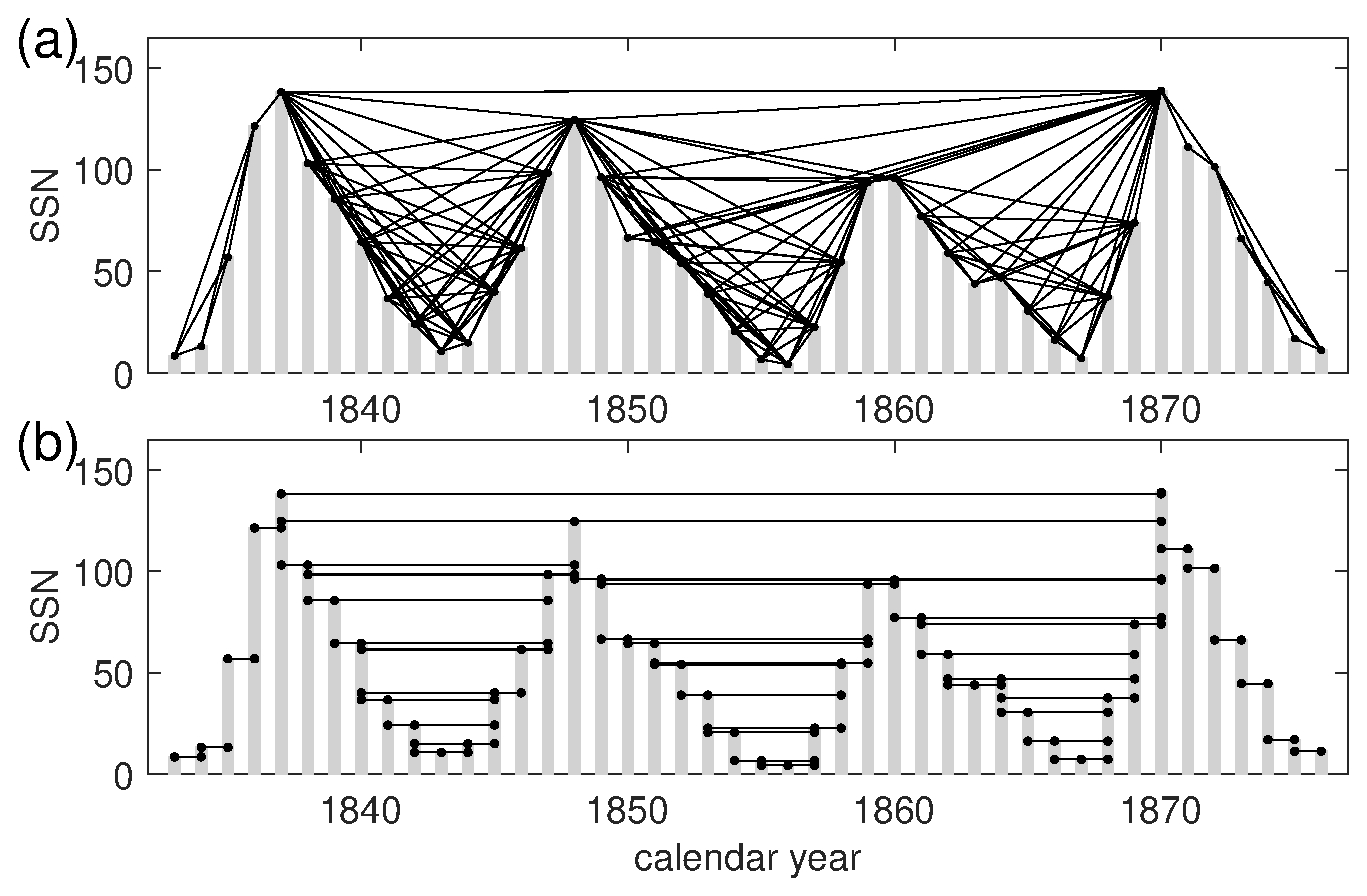
\includegraphics[width=0.8\columnwidth]{Chapter04_VisibilityGt/TSspotnumberYear.eps}
		  \caption{Algorithm of constructing natural visibility graphs (a), and (b) horizontal VG for time series of sunspot number series. Reproduced from \cite{Zou2014}. \label{fig_chap04:timeseriesSS}}
		\end{figure}
		
		\subsubsection{Horizontal visibility graphs}
		As a notable modification of the standard VG algorithm, Luque \textit{et al.} \cite{Luque2009} proposed utilizing a simplified criterion of horizontal visibility for transforming a time series into a complex network. Specifically, they considered two observations made at times $t_i$ and $t_j$ to be connected in a horizontal visibility graph (HVG) if and only if
\begin{align}
x(t_k) < \min \left( x \left(t_i \right), x \left(t_j \right) \right) \label{eq:hvc}
\end{align}
for all $t_k$ with $t_i<t_k<t_j$. 

		The algorithmic difference between HVG and VG is illustrated in Fig. \ref{fig_chap04:timeseriesSS}(b). Note that the geometric criterion defined for the HVG algorithm is more ``visibility restrictive" than its analogous for the standard VG. That is to say, the nodes within the HVG will have ``less visibility" than their counterparts within the VG. It is easily seen that the edge set of the HVG associated with a given time series is a subset of the edge set of the associated VG (i.e., if the horizontal visibility criterion Eq.~(\ref{eq:hvc}) is fulfilled, then also Eq. (\ref{vis_cond}) holds, but not necessarily vice versa). In addition, VGs are invariant under affine transformations of the entire time series, whereas HVGs are not. One notable advantage of HVGs is that they provide an even higher degree of algorithmic simplicity than standard VGs, resulting in the observation that for certain simple stochastic processes and the quasiperiodic transition route to chaos, some basic graph properties can be calculated analytically \citep{Luque2009,Luque2013a,Luque2013d}. On the other hand, the fact that HVGs typically contain a lower number of edges increases the demands regarding the time series length relatively to the standard VG when using this approach in applications such as tests for time-reversal asymmetry \citep{Donges2013}. 
		
		\subsubsection{Other variants of (H)VG}
		Given the definitions of VG and HVG, the resulting graphs are undirected, unweighted. One straightforward generalization of (H)VGs to directional (H)VGs is to introduce directed edges between vertices, i.e., from the cause at $t_i$ to the effect at $t_j > t_i$. As it will be shown in Sec. \ref{sec:timeIRvg}, such directed graphs will give information on time-reversal asymmetry of the considered time series since the connection from $t_i$ to $t_j$ does not necessarily coincident with the connection from $t_j$ to $t_i$. 
		
		There are some further variants of (H)VG depending on the particular properties of the given time series. For instance, given a binary series, in \cite{Ahadpour2012}, a simplified VG has been obtained for binary VG and the visibility condition (expression \eqref{vis_cond}) is reduced to $x(t_i) + x(t_j) > x(t_k)$ that $x(t_k) = 0$ for all $t_k$ such that $t_i < t_k < t_j$. The resulting VG from binary series is always connected and undirected, which is more solvable than the standard VGs. 
		
		Parametric VG has been proposed in \cite{Bezsudnov2014,Snarskii2013a}, introducing "view angle" $\alpha$. When the angle $\alpha = \pi$, the parametric version VG and the standard VG are the same. However, the angle $\alpha = \pi / 2$ does not turn into HVG because $\alpha$ introduces a direction of links in the resulted graphs. The next step is to study the dependence of network structural measures on the parameter $\alpha$. 
		
		Multiscale limited penetrable HVG algorithm has been proposed in \cite{Gao2016,Pei2014a}, which can be regarded as a continuous construction of HVG based on a proper coarse grained time series. In the original HVG, two time points $t_i$ and $t_j$ are connected if no other intermediate points $t_k$ are larger than $\min{(x(t_i), x(t_j))}$, namely, $t_k < \min{x(t_i), x(t_j)}, i < k < j$. Now we use a less restrictive criterion, allowing one of $t_k$ being larger than $\min{(x(t_i), x(t_j))}$, as represented by the new parameter of $L=1$. We allow two points of $t_k$ larger than $\min{(x(t_i), x(t_j))}$ if $L = 2$. When increasing $L$, there are more edges in the resulting HVG comparing to the standard HVG. The standard VG is recovered from HVG if $L \to \infty$. Furthermore, the limited penetrable VG algorithm has been combined with parametric VG in \cite{Li2018}. 
				
		The extension of (H)VGs from a univariate time series to scalar fields has been recently reported in \cite{Xiao2014a,Lacasa2017}, which is conceptually closer to the original idea of visibility graphs. In addition, one may reconstruct (H)VGs for a set of ordered data (either descending or increasing ordered) \cite{Wang2015a}. 
						
		It is also possible to combine the concepts of VGs with transition networks (Sec. \ref{sec:TransitionNt}), for instance, the so-called visibility graphlet approach has been proposed in \cite{Mutua2015,Mutua2016a}. In this case, VGs are constructed respectively for sliding windows and each window is regarded as a network node (phase space partition). The connection between two nodes are decided by the temporal succession. The resulting transition network shows distinct topological features for chaotic series \cite{Mutua2016a}. 
		
		In all above cases, (H)VGs are reconstructed from a given time series. In \cite{Tsiotas2018}, {\textit {Tsiotas et al.}} expanded the VG algorithm to analyze node's attributes of a given graph. More specifically, let us consider a graph $G(V, E)$ and a node-wise attribute $Y$ that might be any of the node-wise network measures, for instance, local clustering coefficient or betweenness centralities. The secondary VG analysis for node-wise attributes $Y$ shows specific ability in pattern recognitions \cite{Tsiotas2018}. 
				
		Other properties of combinatorics have been used to characterize HVGs successfully in \cite{Gutin2011}. Recently, some analytic results have been obtained for some independent and identically distributed random noise, which has exponential degree distribution \cite{Wang2018}. 

		The time complexity of the basic natural VG algorithm is $O(N^2)$, which means that it takes a lot of time when dealing with long time series. A faster transform algorithm has been proposed in \cite{Lan2015a} to reduce the computation time, showing much efficient time complexity $O(N \log N)$. Note that for the HVG algorithm, it is not possible to further improve the computation efficiency because the computation complexity has reached the lower bound $O(N)$. 

	\subsection{Visibility graph properties}
		\subsubsection{Degree distributions}
		Recent work on (H)VGs has mainly concentrated on the properties of the degree distribution $p(k)$ resulting from different kind of processes. Specifically, VGs obtained from periodic signals appear as a concatenation of a finite number of network motifs (given that the basic period is an integer multiple of the sampling rate), i.e., have a regular structure with only a few distinct values of the vertex degree. The opposite extreme case, white noise, yields VGs appearing as exponential random graphs, i.e., random networks characterized by an exponential degree distribution. For example, exponential degree distribution has been tested in wind speed records measured in central Argentina \cite{Pierini2012}. 
		
		In fractal processes, numerical results suggest that $p(k)$ exhibits a power law \cite{Lacasa2008}, $p(k) \sim k^{-\gamma}$. Taking this empirical observation, VG analysis has been suggested to characterize fractional Brownian motions and $f^{\beta}$-noise, finding some heuristic relationship between $\gamma$ and the process Hurst exponent $H$ as $\gamma = 3 - 2H$, and $\gamma = 5 - 2H$ for fractional Gaussian noise \cite{Lacasa2009,Ni2009}. Depending on the fractal properties of the underlying process, recently an algorithm for constructing VGs from segmented time series has been proposed \cite{Ahmadlou2012}, which estimates power-law exponents reflecting scale-free properties quite well. The idea hinges on a proper choice of the time delay $\tau$, which re-samples the original time series resulting in a number of segmentations. However, the number of segments to be used is often not known in the original algorithm. In other words, we do not know the upper bound of $\tau_{max}$ to terminate the computation. So far, only a heuristic choice of $\tau_{max}$ has been suggested when network characteristics of segmented time series show more or less convergent behavior \cite{Ahmadlou2012}. This improved algorithm has been applied to diagnose Autism spectrum disorders \cite{Ahmadlou2012}. Since there are much concerns regarding the statistical justification of the power laws of VGs, one can directly analyze the degree sequence (instead of the distribution) by detrended fluctuation analysis \cite{Czechowski2016}, which quantifies multifractal properties better than the standard VGs analysis.  
	
		Some exact results of $p(k)$ of the HVG associated with generic uncorrelated random series have been obtained in \cite{Luque2009}. More specifically, for a bi-infinite time series created from a random variable $X$ with probability distribution $f(x)$ with $x\in [0, 1]$, it has been proved that the degree distribution of the graph has an exponential form 
		\begin{equation}\label{pkhvg}
		p(k) = \frac{1}{3} (\frac{2}{3})^{k-2}, 
		\end{equation}
where $k$ is the degree. Interestingly, every probability distribution $f(x)$ of uncorrelated random series have the same exponential form. Numerical results of $f(x)$ from a uniform, a Gaussian and a power law form (e.g., $f(x) \sim x^{-2}$) show perfect agreements with this theoretical predictions \cite{Luque2009}. A general diagrammatic theory has been proposed in \cite{Lacasa2014b} to compute $p(k)$ for any given dynamical process with well defined invariant measure. Taking into account the time information explicitly as in so-called directed HVG (as will be explained below), the outgoing degree distribution $p_{out}(k) = (1/2)^{k}$. Further solvable example are Markovian processes with an integrable invariant measure $f(x)$, for instance, the stationary Ornstein-Uhlenneck process, one dimensional chaotic and quasiperiodic maps of with smooth invariant measure. In addition, the mean degree $\bar{k}$ of the HVG associated to an uncorrelated random process is then given by 
\begin{equation}
\bar{k} = \sum k p(k) = \sum_{k=2}{\infty} \frac{k}{3}{(\frac{2}{3})}^{k-2} = 4.
\end{equation}
For an infinite periodic series of period $T$, the mean degree $\bar{k}$ is $\bar{k} = 4 ( 1 - \frac{1}{2T})$. 
	
		Nevertheless, similar to VGs, HVGs have been successfully applied to studying time series from various fields of sciences. Within the area of the present manuscript, we particularly notice the recent paper by \cite{Yu2012} who studied the multifractal properties of some solar flare index in terms of HVG characteristics. The properties of HVG have been tested in river flows \cite{Braga2016}, showing exponential degree distributions. 
		
		In order to understand the hypothetical scale-free property of $p(k)$ for VGs from fractal records, one has to note that typically, maxima of the time series have visibility contact with more other vertices than other points, i.e., hubs of the network often form at maximum values of the recorded observable. Put it differently, the degree of a vertex in the VG characterizes the maximality property of the corresponding observation in comparison with its neighborhood in the time series. Although local large time series values have better visibility than other small values, hub nodes of large degrees of VGs do not necessarily correspond to higher values, especially when there are some sort of periodic trends in the given data sequence, for instance wind speed records \cite{Pierini2012,Zou2014a}. Therefore, the relationship between maxima time series points and hubs of VGs is not completely general, since there can be specific conditions (e.g., a concave behavior over a certain period of time) which can lead to highly connected vertices that do not coincide with local maxima, for example, in case of a Conway series \cite{Lacasa2008}. 
				
		In addition, minima of time series provide complementary insight for the understanding of the particular process, for instance, sun spot series \cite{Zou2014a}. In the standard VGs, the contributions of local minimum values have been somehow largely overlooked by degree distribution $p(k)$ because minimum values are basically non-hubs. One simple solution is to study the negatively inverted counterpart of the original time series, namely, $-x(t_i)$, which quantifies the properties of the local minima \cite{Zou2014a}. For convenience, we use $k_{-x}$ and $p(k_{-x})$ to denote degree sequence and distribution of VG resulted from $-x(t_i)$. Here, we remark that this simple inversion of the time series allows us to create an entirely different complex network. This technique has demonstrated to be useful to understand the long-term behavior of strong minima of the solar cycles \cite{Zou2014a}. We will review these results in Sec. \ref{subsec:sunnum}. 
		
		Based on degree distribution $p(k)$, we can calculate the graph entropy $h = - \sum_{k} p(k) \log p(k)$, which is used as the approximation to the Shannon entropy $H$ of the corresponding time series $x(t)$ \cite{Luque2016,Goncalves2016}. Furthermore, the VG aggregation operator has been proposed in \cite{Chen2014,Jiang2016}. This operator includes the temporal information in the weights of the aggregation, showing computational simplicity comparing to other traditional aggregation operators.  
					
		\subsubsection{Stochastic vs. deterministic dynamics}
		Concerning the HVG, exponential functional forms have been obtained for many random processes, namely, $p(k) \sim e ^{-\lambda k}$. A scaling factor of $\lambda_c = \ln (3/2)$ has been found in the case of uncorrelated noise (white noise), which has been further proposed to separate stochastic from chaotic dynamics in the following senses \cite{Lacasa2010,Lacasa2014b,Ravetti2014}: (i) correlated stochastic series are characterized by $\lambda > \lambda_c$, slowly tending to an asymptotic value of $\ln (3/2)$ for very weak correlations, whereas (ii) chaotic series are often characterized by $\lambda_{chaos} < \lambda_c$ for decreasing correlations or increasing chaos dimensionality, respectively \cite{Lacasa2010}. In \cite{Zhang2017}, we have provided some further examples supporting argument (i). Meanwhile, we showed some peculiar results indicating that $\lambda_c$ should not be interpreted as a general critical value separating chaos from noise. 
		
		Let us focus on applying (H)VG analysis to auto-regressive (AR) stochastic processes, which often describe certain time-varying processes in nature, economics, etc. The AR model specifies that the output variable depends linearly on its own previous values and on a stochastic term. More specifically, ${\bf x} = [x_1, x_2, \ldots, x_i, \ldots, i \in \mathbb{Z} ]$ is an AR model of order $p$ denoted as AR($p$) if
\begin{equation} \label{def:AR}
x_t = \sum_{j=1}^{p}\varphi_j x_{t-j} + \varepsilon_t, 
\end{equation}
where $\varphi_j, j \in [1, p],$ are real-valued coefficients of the model, and $\varepsilon_t$ is white noise. We further assume that the error terms $\varepsilon_t$ follow a Gaussian distribution with zero mean and unit variance. Specifically, we perform both VG and HVG analysis for AR(1), namely, (i) $|\varphi_1| < 1$ for the AR(1) model. It is known that $\varphi_1 > 0$ corresponds to positive correlation and the correlation length increases when $\varphi_1$ is increased from 0 to 1. In contrast, anti-correlation is observed for negative coefficient $\varphi_1$. Similar H(VG) analysis for the AR(2) model have reported in \cite{Zhang2017}. 

		In the case of $\varphi_1 > 0$, we find that $p(k)$ approximately follows an exponential distribution. To illustrate this finding, the cumulative degree distributions $F(k)$ for $\varphi_1 = 0.3 $, $0.9$ and $-0.5$ are shown in Fig. \ref{fig:lambda_AR1}A and B, where clear scaling regimes are present in the semi-log plots. Furthermore, when increasing $\varphi_1$, in the VG, the exponent $\lambda$ shows a monotonically decreasing trend (Fig. \ref{fig:lambda_AR1}C). In contrast, the value $\lambda$ for the HVG is increased (Fig. \ref{fig:lambda_AR1}D). The result of Fig. \ref{fig:lambda_AR1}D confirms the hypothesis stated in \cite{Lacasa2010} the all $\lambda$ should be larger than $\lambda_c = \ln (3/2)$ as the correlation length is increased in the case of positively correlated increments.
\begin{figure}
	\centering
	\includegraphics[width=\columnwidth]{Chapter04_VisibilityGt/ar1_positive_lambda_vg_hvg.eps}

\caption{(color online) (A, B) Estimates of $\lambda$ for approximately exponential degree distributions of AR$(1)$ process. (C, D) $\lambda$ versus $\varphi_1$. (A, C) VG, and (B, D) HVG. When $\varphi_1>0$, $\lambda$ has a decreasing trend in the VG, while in the HVG, $\lambda$ rises when the correlation length increases. Each dot in panels C and D represents an average over 50 independent random realizations of 5000 data points. In (D), $\lambda$ values smaller than $\ln 3/2$ are highlighted by red color. \label{fig:lambda_AR1}}
\end{figure}

		In turn, when $\varphi_1 < 0$, we observe some peculiar results that seem to contradict the hypothesis stated in \cite{Lacasa2010}. According to this hypothesis, $\lambda$ should be larger than $\lambda_c$ ($\lambda > \lambda_c$) in stochastic processes in contrast to $\lambda < \lambda_c$ for chaotic maps. The results of Fig. \ref{fig:lambda_AR1}D do not support this claim when $\varphi_1$ is negative in the AR(1) model. Instead, we find a region where the slope of the exponential degree distribution is smaller than $\ln (3/2)$ (as highlighted in Fig. \ref{fig:lambda_AR1}D). This suggests that the critical value of $\ln (3/2)$ should not be understood as a general law of separating correlated stochastic from chaotic processes, which requires further investigation. 

		Working with correlated stochastic time series, further results in \cite{Manshour2015} do not adequately support the arguments of exponential degree distributions as reported in \cite{Lacasa2010}. Moe specifically, they have constructed (H)VGs for fractional time series with three different methods, a generic $1 = 1 / f^{\beta}$ noise with Fourier filtering method, a deterministic fBm process of Weierstrass-Mandelbrot function, and a stochastic fBm process with successive random addition method. The numerical analysis show that VG algorithm may not be a well-defined method to extract correlation information of a time series and its statistics is not essentially the same as that of the HVG. The degree distributions of HVGs are shown to have parabolic exponential forms with Hurst dependent fitting parameter \cite{Manshour2015}. Therefore, we conclude that hypothesis of \cite{Lacasa2010,Lacasa2014b,Ravetti2014} needs careful numerical simulations for proper interpretations. 
			
		\subsubsection{Local network properties}
		Here, we consider other local network properties besides degrees and their distributions. In the case of VGs, the local clustering coefficient $\mathcal{C}_i$ and its relationship with the degree $k_i$ have been numerically studied recently in human heartbeat data \cite{Shao2010}. Particularly, it has been observed that $\mathcal{C}(k) \sim k^{-\gamma}$ and $\gamma = 1$, pointing to a hierarchical organization of the network \cite{Albert2002}, since vertices $i$ with high $\mathcal{C}_i$ and low $k_i$ (which are most abundant) form densely connected subgraphs, indicating a strong modular structure of the VG. 

		In the case of HVG associated with an uncorrelated random series, the local clustering coefficient $\mathcal{C}_i$ can be easily deduced by means of geometrical arguments. For a given node $i$, $\mathcal{C}_i$ denotes the rate of nodes connected to $i$ that are connected between each other. In other words, we have to calculate from a given node $i$ how many nodes from those visible to $i$ have mutual visibility (triangles), normalized with the set of possible triangles $\binom{k}{2}$, where $k$ is the degree of node $i$. Based on a general rule between degree $k$ and local clustering coefficient
		\begin{equation}
		\mathcal{C}_i(k) = \frac{k-1}{\binom{k}{2}} = \frac{2}{k}, 
		\end{equation}
one obtains the local clustering coefficient distribution $p(\mathcal{C})$ as 
		\begin{equation}
		p(\mathcal{C}) = \frac{1}{3} (\frac{2}{3})^{2/\mathcal{C} -2}. 
		\end{equation}
The above theoretical result has been confirmed by uncorrelated random series \cite{Luque2009}. In addition, for HVG of a binary sequence, $p(\mathcal{C})$ has a simplified expression as reported in \cite{Ahadpour2012}. 
			
		In many cases local maxima of the underlying time series are expected to have large values of betweenness because high values often correspond to hubs in VGs which separate different parts of the series without mutual visibility contact and, thus, act as bottlenecks in the network structure, bundling a large number of shortest paths between vertices at $t < t_i$ and $t > t_i$, respectively. However, in contrast to the degree, betweenness is additionally affected by the vertex' position in the underlying time series due to a simple combinatorial effect: Considering that the majority of shortest paths that cross a vertex $i$ connect observations before and after $i$ with each other, there are more possible combinations of such points for $i$ being close to the middle of the time series than for vertices close to the edges of the record. In this respect, in a VG betweenness centrality of a vertex mixes information on the local maximality of the corresponding observation and its position within the time series.
		
		In the case of closeness centrality the position of a vertex in the time series is even more important in comparison with the value of the underlying observable. Specifically, this measure is strongly determined by the number of vertices to its left and right, respectively. In this spirit, it can be argued that in the middle of the time series, high closeness values are more likely than at its ends. As argued above, a similar (but weaker) effect contributes to betweenness and - close to the edges of the record - also to the degree (consequently, the highest degree and betweenness values can be taken by other vertices than that corresponding to the global maximum). In contrast, the local clustering coefficient is almost unaffected except for vertices very close to the beginning and end of the time series, since direct connectivity is mainly established between vertices that correspond to observations that are not very distant in time. 
		
		We note that boundary effects play an important role in the computation of the above centrality measures as that has been numerically reported in \cite{Donner2012}. In particular, it has been shown that the local clustering coefficient is almost unaffected, but the impact of boundaries on the estimated vertex properties is particularly strong for short records, which are typical in geophysical applications. Specifically, degree and other centrality properties of observations close to both ends of a time series are systematically underestimated, which may artificially alter the interpretation of the corresponding results in their geophysical context. Hence, a careful treatment and interpretation of the results of VG analysis is necessary in such cases \cite{Donner2012}.
	
				
		\subsubsection{Global network properties}
		In contrast to other approaches to complex network based time series analysis, in a VG the edge density $\rho$ is a true network characteristic rather than a parameter of the method (cf. \cite{Donner2010a,Donner2011}) for the corresponding meaning for recurrence networks). Specifically, a maximum edge density of 1 would be present if the underlying time series is globally convex (e.g., of regular parabolic shape), whereas low values indicate a strong fragmentation of the VG and, hence, irregularity of fluctuations of the underlying observable. 
		
		For a holistic characterization of a graph, $\mathcal{C}$ and $\mathcal{L}$ have attracted particular interest, since their common behavior gives rise to a mathematical evaluation of the small-world phenomenon, i.e., the emergence of real-world networks with a high degree of clustering and a short average path length \cite{Watts1998}.
		
		The topological properties of HVGs constructed from fractional Brownian motions with different Hurst indexes $H \in (0, 1)$ have been reported in \cite{Xie2011}. It is found that the clustering coefficient $\mathcal{C}$ decreases when $H$ increases. 
		
		It can be expected that the value of $\mathcal{L}$ is large when there are only few edges in the VG (low edge density) and low for a high edge density. Hence, average path length and edge density capture essentially similar properties of the underlying time series. For uncorrelated random series, the mean path length $\mathcal{L}$ of HVG has a logarithmic scaling relationship with the length of time series $N$, in particular, $\mathcal{L}(N) = 2 \ln (N) + 2 (\gamma - 1) + O(1/N)$, where $\gamma$ is the Euler-Mascheroni constant \cite{Luque2009}. In the case of fractional Brownian motions with different Hurst indexes $H \in (0, 1)$, and for fixed length of time series of $N$ points, $\mathcal{L}$ increases exponentially with $H$. In addition, $\mathcal{L}$ increases linearly with respect to $N$ when $H$ is close to 1 and in a logarithmic form when $H$ is close to 0 \cite{Xie2011}. 
	
		Besides studies on the small-world effect, the assortativity of VGs has recently attracted considerable interest. Specifically, the presence of assortative behavior implies so-called hub attraction, whereas disassortative behavior relates to hub repulsion. It has been shown that the latter is a necessary condition for the emergence of fractal structures in networks \cite{Song2006}. For example, for Brownian motion (a fractal stochastic process), hub repulsion is not present, and the resulting VGs are non-fractal, but show a scaling of the average path length with increasing net-work size as $\mathcal{L}(N)\sim \log N$, which is typical for small-world networks. In contrast, for the Conway series (a deterministic fractal) one finds hub repulsion and $\mathcal{L}\sim N^{-\beta}$, which implies the presence of a fractal VG (Lacasa et al. 2008). In this respect, the assortativity coefficient or, more specifically, the scaling of the degree correlation determines the fractality of a VG \cite{Song2006}, which is an interesting and potentially relevant property when studying fractal time series.		
	
		Of course, beyond the aforementioned characteristics there are multiple other measures one could also consider for describing the properties of VGs. This includes also measures characterizing the properties of individual edges as well as the distributions of small subgraphs (motifs). For example, the consideration of four-node subgraphs helps to show different dominant motifs ranks in the VGs of human ventricular time series, which distinguishes ventricular fibrillations from normal sinus rhythms of a subject \cite{Li2011}. Furthermore, the profiles of sequential $n$-node motifs of (H)VGs appear with characteristic frequencies which have been computed analytically for certain deterministic and stochastic dynamics \cite{Iacovacci2016}. 
		
		\subsubsection{Practical considerations}
		Many recent publications on (H)VG analysis of time series have particularly made use of data from model systems, which are characterized by rather ideal conditions for statistical analysis. Even for most practical applications presented so far, the properties of the data under study have allowed using this methodological approach without extensive precautions. However, when operating with data obtained in a geophysical context, features challenging basically any kind of time series analysis are often present, including missing data, heteroscedastic ``noise", or even uncertainties in the time domain (the latter being particularly relevant in paleo-climatology). The explicit treatment of the resulting effects on VG properties has not yet been investigated elsewhere \cite{Donner2012}. 

		As in the previous section, in the following a corresponding study is presented for the specific case of a Gaussian white noise process as a simple, but still illustrative example. It has to be emphasized that for ``real" data characterized by a non-Gaussian probability distribution function, serial dependences, or even (multi-)fractal behavior, the resulting effects could well be much stronger than in this example. A detailed study of the interdependences between such features of the data and the resulting effects of missing data and uncertainties on VG properties is, however, beyond the scope of the presented research.

		{\bf{Missing data}} 
		One important problem of many observational time series - not only in geophysics - is the presence of missing data. Since existing methods of time series analysis typically require a uniform spacing in time, this problem is most often addressed by means of interpolation or sophisticated imputation of the missing observations. In general, there is a great variety of possible approaches for such gap filling, which shall not be further discussed here. Specifically, it is not always a priori clear what method performs best under the specific conditions of the data studied.
		
		As far as VGs are concerned, the problem of missing data has not yet been explicitly addressed. Unlike many other approaches of time series analysis VGs do not explicitly require uniform sampling. Hence, missing data could be ignored when performing a corresponding analysis. However, if it is known that there must have been an observation at a given time, it could be conceptually problematic to neglect this information in the analysis. From a broader perspective, it can be argued, however, that this argument applies to all kinds of time series, since values of the considered observable (with a continuous-time variability) taken in between two subsequent observations remain always unknown, but could have a certain impact on the results of the analysis. 
		
		Looking at the issue of missing values from a complementary perspective, one can reinterpret this problem as an attack to (or just failure of) the complex network represented by the visibility graph. In complex network theory, the impact of such attacks on various types of networks has been intensively studied under the aspect of safety and robustness of infrastructures (e.g., Albert et al. 2000, Holme et al. 2002). In general, one has to distinguish random failures (corresponding to randomly miss-ing values) from intentional attacks, which typically affect the network hubs. Since for a VG, these hubs correspond to the maxima of the under-lying time series, this effect is particularly relevant for certain types of censored data, e.g., in case of measurement failures due to the limited de-tection range of a measurement device. Since is known that attacks on hubs typically have a more severe effect on the network architecture than other vertices, censoring can strongly alter the properties of the resulting VGs. However, even a random removal can have notable consequences for the VG properties on both global and local scale.
		
		In order to illustrate the effect of missing data on the properties of VGs, in the following, two different types of treatment are studied, which can be considered as opposite extreme cases. On the one hand, missing data will be simply neglected in the generation of the VG. On the other hand, since there is no information about the magnitude of the missing values, it can be a more honest solution to consider the VG as being fragmented into pieces corresponding to times before and after the missing observation, i.e., regarding the VG becoming decomposed into mutually disconnected subgraphs. It should be noted, however, that the latter approach results in the emergence of additional boundary effects. It should be emphasized that sophisticated gap filling by means of interpolation or imputation will be most likely a better strategy in many practical applications. 

		{\bf{Homo- and heteroscedastic uncertainties}} In a similar way as for the treatment of missing values, the influence of measurement uncertainties on the resulting VG properties can be studied. For convenience, homoscedastic uncertainties are modeled as an additional additive Gaussian white noise component ({\color{red} figure 8?}), whereas the heteroscedastic case is studied by considering multiplicative noise with a reasonable, simple analytical distribution ({\color{red}Figure 9?}). Again, it is found that in both cases the signal-to-noise ratio has a considerable effect by systematically shifting the distributions of vertex properties obtained for the original data towards those expected for the noise process. Note that since in the considered numerical example both signal and noise originated from mutually independent Gaussian white noise processes, there is a saturation of the KS statistics for moderate noise at values corresponding to the variance of VG properties for independent realizations of the same ``signal" process.
		
		
		{\bf{Uncertain timings}} 
		In full analogy to the case of uncertainties in the observable $x$, one can study the impact of uncertain timings $t$ on the properties of the resulting VGs. The latter is a wide-spread problem particularly in the analysis of paleoclimate time series \cite{Telford2004}. Since in the construction of VGs both observable and time enter in terms of an inequality defined by a linear relationship, it is not surprising that uncertain timing can indeed have a similar effect on the VG properties as uncertainties in the measurement itself. Figure 10 displays the corresponding results for a realization of Gaussian white noise originally observed with regular spacing, with the timings being corrupted later as
		\begin{equation}
		\tilde{t_i} = t_i + \Delta t (| 1 - 2\eta_i | - 0.5).
		\end{equation}		
		Here,  $\eta_i$ are independent realizations of a random variable with uniform distribution in $[0,1]$, and $\Delta t$ is the spacing between subsequent observations in the original data set. Note that this specific form of the time-scale corruption, which allows preserving the temporal order of observations, has been inspired by the tent map as a paradigmatic nonlinear mapping often used as an illustrative example in complex systems sciences. The obtained results demonstrate that the distribution of vertex properties of a VG are indeed affected by modifications of the time-scale, however, the changes are considerably smaller than for noisy corruptions of the measurements themselves. The reason for this is that the modification used here has been restricted by the normal sampling interval, whereas the changes induced by additive and multiplicative noise allowed for comparably larger modifications in the data.
			
		{\bf{Point process}}
		Point processes are ubiquitous in geophysics, for instance, seismic magnitude series \cite{Telesca2012}. A point process is often characterized by random time occurrence of the events and these events are clusterized because the events are neither Poissonianly nor regularly distributed over time. To check the effects of irregular timing on degree distributions, they construct two VGs from (1) the seismic series of the original random occurrence times, and the series (2) that has been substituted by regular conventional time unit. Interestingly, almost identical results have been obtained for the degree distributions, which suggests that the effects of irregular timing are not crucial. 

		The trivial connection of neighboring points in time in the (H)VG enhances the signature of structures due to autocorrelations in the record under study. Although this might be desirable for (H)VGs since some of their respective network properties are explicitly related with the presence of serial dependences (e.g., the typical scale of the degree distribution of HVGs, cf. \cite{Luque2009}), there could be situations in which one is interested in removing the corresponding effects. In such cases, it is possible to introduce a minimum time difference for two observations to be connected in the network for removing the effect of slowly decaying auto-dependences, which would correspond to the Theiler window in other concepts of nonlinear time series analysis (\cite{Theiler1986}).

		{\color{red}General question: What information can be gained from VGs? Which networks properties are (when) useful to study? }

	\subsection{Bivariate visibility graph methods}
	Despite the success, the range of applicability of (H)VGs methods has been mainly limited to univariate time series, although the most challenging problems in the area of nonlinear science concern systems that are described by multivariate time series. We can do synchronization analysis when generalizing (H)VG analysis from a univariate to bivariate time series \cite{Ahmadlou2012a,Mitra2012}. Furthermore, cross visibility algorithm helps to understand coupling and information transfer between two time series \cite{Mehraban2013}. We summarize some different approaches to characterize bivariate (H)VGs. 
	
		\subsubsection{Visibility graph similarity}
		Based on the definition of HVGs, Lacasa \textit{el al.} \cite{Lacasa2015b} proposed to transforming a multidimensional time series into an appropriately defined multiplex visibility graph. New information can be extracted from the original multivariate time series, with the aims of describing signals in graph-theoretical terms or to construct novel feature vectors to feed automatic classifiers in a simple, accurate and computationally efficient way. 
		
		Consider a $M$-dimensional real valued time series $\{{\bf{x}}(t) \}_{t=1}^{n}$, with ${\bf{x}}(t) = (x^{[1]}(t), x^{[2]}(t), \dots, x^{[M]}(t)) \in \mathbb{R}^M$ for any value of $t$, measured empirically or extracted from a $M$-dimensional, either stochastic or deterministic dynamical system. An $M$-layer multiplex visibility graph $\mathcal{M}$ is then constructed, where layer $\alpha$ corresponds to the HVG associated to the time series of state variable $\{ x^{[\alpha]}(t) \}_{t=1}^{N}$. Note that $\mathcal{M}$ is represented by the vector of adjacency matrices of its layers $\mathcal{A} = \{A^{[1]}, A^{[2]}, \dots, A^{[M]}\}$, where $A^{[\alpha]} = \{a_{ij}^{[\alpha]} \}$ is the adjacency matrix of layer $\alpha$. Such a mapping builds a bridge between multivariate series analysis and the recent developments in the theory of multilayer networks \cite{Boccaletti2014}, making it possible to employ the structural descriptors introduced to study multiplex networks as a toolbox for the characterisation of multivariate signals. 
		
		Two measures have been proposed to capture, respectively, the abundance of single edges across layers and the presence of inter-layer correlations of node degrees \cite{Lacasa2015b}, which help to characterize information shared across variables (layers) of the underlying high dimensional system. Simply speaking, we compute these two measures by Eqs. (\ref{eq:RNmultiplex}, \ref{eq:RNmultiplexW}) based on the adjacency matrices of HVGs. More specifically, the first measure is the average edge overlap (Eq. \eqref{eq:RNmultiplexW}),  	
%		The first measure is the average edge overlap
%\begin{equation} \label{eq:VGmultiplexW}
%\omega = \frac{\sum_i\sum_{j>i} \sum_{\alpha}a_{ij}^{[\alpha]}}{M \sum_i\sum_{j>i}(1-\delta_{0, \sum_{\alpha}a_{ij}^{[\alpha]}})}
%\end{equation}
which computes the expected number of layers of the multiplex on which an edge is present. Note that $\omega$ takes values in $[1/M, 1]$ and in particular $\omega = 1/M$ if each edge $(i, j)$ exists in exactly one layer, i.e. if there exist a layer $\alpha$ such that $a_{ij}^{[\alpha]} = 1$ and $a_{ij}^{[\beta]} = 0 \forall \beta \neq \alpha$, while $\omega = 1$ only if all the $M$ layers are identical. As a consequence, the average edge overlap of a multiplex VG can be used as a proxy of the overall coherence of the original multivariate time series, with higher values of $\omega$ indicating high correlation in the microscopic structure of the signal. 

		The second measure proposed in \cite{Lacasa2015b} is to quantify the presence of interlayer correlation between the degrees of the same node at two different layers. More specifically, given a pair of layers $\alpha$ and $\beta$ of $\mathcal{M}$, respectively characterized by the degree distributions $P(k^{[\alpha]})$ and $P(k^{[\beta]})$, the interlayer correlation is defined by the mutual information $I_{\alpha, \beta}$ (Eq. \eqref{eq:RNmultiplex}) % as 
%		\begin{equation} \label{eq:VGmultiplex}
%		I_{\alpha, \beta} = \sum_{k^{[\alpha]}} \sum_{k^{[\beta]}} P(k^{[\alpha]}, k^{[\beta]}) \log \frac{P(k^{[\alpha]}, k^{[\beta]})}{P(k^{[\alpha]}) P(k^{[\beta]}) }, 
%		\end{equation}
		where $P(k^{[\alpha]}, k^{[\beta]}) $ is the joint probability to find a node having degree $k^{[\alpha]}$ at layer $\alpha$ and degree $k^{[\beta]}$ at layer $\beta$. The higher $I_{\alpha, \beta}$ the more correlated the degree distributions of the two layers and therefore the structure of the associated time series. Then the average of $I_{\alpha, \beta}$ over every pair of layers of $\mathcal{M}$ gives a scalar variable $I = \left < I_{\alpha, \beta}\right>_{\alpha, \beta}$, which captures the amount of information flow in the multivariate time series. 
		
		Note that the second measure above gives a weighted correlation matrix of $M \times M$ and each entry is represented by $I_{\alpha, \beta}$. That means the original $M$-dimensional time series is transformed to a weighted graph of $M$ nodes, where each node represents one layer and the weights of the edge denote the magnitude of mutual information computed from the associated (H)VG degree distributions.  
						
		\subsubsection{Joint and excess degrees} \label{subsec:jointdegreeVG}
		In addition, we introduce some network-theoretic quantities to quantify the asymmetries in bivariate time series \cite{Zou2014}. Following the notations as described for multiplex (H)VG, we restrict our analysis with $2$-dimensional time series which resulting two layers $\alpha$ and $\beta$. For $\{x^{[\alpha]}(t)\}_{t=1}^{N}$ and $\{x^{[\beta]}(t)\}_{t=1}^{N}$, we again denote two (H)VGs with adjacency matrices $A^{[\alpha]}$ and $A^{[\beta]}$, respectively. Note that the sets of vertices are the same for both subgraphs, with differences exclusively in the set of edges.

Based on the thus obtained (H)VGs, we proceed as follows:
\begin{enumerate}
\item From the two (H)VGs, we have two sets of neighbors, $\mathcal{N}_{x^{[\alpha]}, x^{[\beta]}}(t) = \left\{ A_{t, t_j}^{{[\alpha]}, {[\beta]}} \equiv 1, t_j \in \left\{1,\ldots, N \right\}/\left\{t\right\} \right\}$ for each time $t \in \left\{1,\ldots, N \right\}$. The \textit{degree sequences} are then defined as
\begin{align}
&k_{{[\alpha]}, {[\beta]}}(t) = \# \mathcal{N}_{{[\alpha]}, {[\beta]}}(t) = \sum_{t_j} A_{t,t_j}^{{[\alpha]}, {[\beta]}}(t).
\end{align}

\item The \textit{joint degree sequence}
\begin{align} \label{eq:jointK}
&k^{joint}(t) = \# \left( \mathcal{N}_{{[\alpha]}}(t) \cap \mathcal{N}_{{[\beta]}}(t) \right) = \sum_{t_j} A_{t,t_j}^{{[\alpha]}}(t)\cdot A_{t,t_j}^{{[\beta]}}(t).
\end{align}
gives the number of common neighbors of a vertex corresponding to time $t$ in both sequences.

Notably, we can define $k^{joint}(t)$ as the degree sequence of a \textit{joint (horizontal) visibility graph} combining the visibility criteria for two distinct time series. Here, the adjacency matrix is defined by the point-wise multiplication of the individual (H)VGs' adjacency matrices. This idea is conceptually related to the concept of joint recurrence plots encoding the simultaneous recurrence of two dynamical systems in their respective phase spaces \cite{romano2004}. As in the latter case, generalizing joint (H)VGs to the case of more than two time series is straightforward, but will not be considered here given the bivariate nature of the data under study.

\item In a similar spirit as the joint degree sequence, we can quantify the number of edges associated with time $t$, which connect to vertices contained in $\mathcal{N}_{x^{[\alpha]}}(t)$ but \textit{not} in $\mathcal{N}_{x^{[\beta]}}(t)$, or vice versa. More specifically,
\begin{align}
k_{{[\alpha]}}^{O}(t) & = \# \left( \mathcal{N}_{{[\alpha]}}(t) \cap \overline{\mathcal{N}_{{[\beta]}}(t)} \right)  =  \sum_{t_j} A_{t,t_j}^{{[\alpha]}}(t)\cdot \left( 1-A_{t,t_j}^{{[\beta]}}(t) \right) \\
k_{{[\beta]}}^{O}(t) & = \# \left( \mathcal{N}_{{[\beta]}}(t) \cap \overline{\mathcal{N}_{{[\alpha]}}(t)} \right) = \sum_{t_j} A_{t,t_j}^{{[\beta]}}(t)\cdot \left(1-A_{t,t_j}^{{[\alpha]}}(t) \right)
\end{align}
(where $\overline{\mathcal{N}_{{[\alpha]}, {[\beta]}}(t)}=\{1,\ldots,T\}\cap \left\{ \mathcal{N}_{{[\alpha]}, {[\beta]}}(t)\cup t\right\}$ is the complementary set of $\mathcal{N}_{{[\alpha]}, {[\beta]}}(t)$) measures the number of neighbors that belong \textit{only} to $\mathcal{N}_{{[\alpha]}}(t)$ or $\mathcal{N}_{{[\beta]}}(t)$, respectively. In what follows, $k_{{[\alpha]}, {[\beta]}}^{O}(t)$ will be referred to as the \textit{conditional degree sequences}. By definition,
\begin{align}\label{eq:nad}
k_{{[\alpha]}, {[\beta]}}^{O}(t)=k_{{[\alpha]}, {[\beta]}}(t)-k^\textrm{joint}(t).
\end{align}
\end{enumerate}

Based on the latter definitions, we can proceed in a similar way as in Eq.~\eqref{eq:nad} and compute the following properties:
\begin{align} \label{eq:deltaK}
\Delta k(t) &= k_{{[\alpha]}}^{O}(t) - k_{{[\beta]}}^{O}(t) = k_{{[\alpha]}}(t) - k_{{[\beta]}}(t) \\ \label{eq:deltaReK}
\Delta_{rel} k(t) &= \Delta k(t)/\left(k_{{[\alpha]}}(t) + k_{{[\beta]}}(t) \right).
\end{align}
The \textit{excess degree} $\Delta k(t)$ quantifies how much ``more convex'' the fluctuations of $A^{[\alpha]}$ are in comparison with $A^{[\beta]}$ around a given time $t$ (i.e., how many more or less visibility connections the observation of $A^{[\alpha]}$ at time $t$ obeys in comparison with $A^{[\beta]}$). By additionally considering the \textit{relative excess degree} $\Delta_{rel} k(t)$ normalized by the sum of the individual degrees, we obtain a measure that does not exhibit marked sensitivity with respect to the actual degrees $k_{{[\alpha]}, {[\beta]}}$, which may considerably vary over time according to the statistical and dynamical characteristics of the data.

In  Sec. \ref{subsec:sunspotsAsym}, we will summarize the applications of $\Delta k(t)$ and $\Delta_{rel} k(t)$ to characterize the North--South asymmetry of solar activity \cite{Zou2014}, which provide many nonlinear properties that have not been obtained by other methods. Notably, our approach is conceptually related with recently developed (H)VG-based tests for time series irreversibility, which compare (among others) degree distributions obtained when considering edges to past and future observations separately \citep{Donges2013}.


	\subsection{Decomposition of visibility graphs} \label{sec:timeIRvg}
		\subsubsection{Time-directed visibility graphs and characterizations}
		So far in the literature the family of visibility graphs are undirected, as visibility did not have a predefined temporal arrow. These can be made directed by again assigning to the links a time arrow, which result in the so called directed VGs (DVGs) and directed HVGs (DHVGs). Accordingly, a link between $i$ and $j$ (where time ordering yields $i< j$) generates an outgoing link for $i$ and an ingoing link for $j$. Therefore, the degree $k(t)$ of the node $t$ is now split into an ingoing degree $k_{in}(t)$, and an out-going degree, such that $k(t)= k_{in}(t)+k_{out}(t)$. The ingoing degree $k(t)$ is defined as the number of links of node $t$ with other past nodes associated with data in the series (that is, nodes with $ t' < t$). Conversely, the outgoing degree $k_{out}(t)$, is defined as the number of links with future nodes. {\color{red}A graph illustration of the method?} Then we define the \textit{in} and \textit{out} (or ingoing and outgoing) degree distributions of a DVG (DHVG) as $P_{out}(k) \equiv P(k_{out} = k)$ and $P_{in}(k) \equiv P(k_{in} = k)$, respectively. An important property at this point is that the ingoing and outgoing degree sequences are interchangeable under time series reversal. 
		
		Given the adjacency matrix $A_{ij}$ of a (H)VG, the degree {$k_i =\sum_{j} A_{ij}$} measures the number of edges incident to a given vertex {$i$}. Then, Donges \textit{et~al.} \cite{Donges2013} used different notations for in- and out-degree sequences. More specifically, they decompose this quantity $k_i$ for a vertex corresponding to a measurement at time $t_i$ into contributions due to other vertices in the past and future of $t_i$,
\begin{eqnarray} \label{eq:kvin}
k_i^r &= \sum_{j<i} A_{ij},\\ \label{eq:kvout}
k_i^a &= \sum_{j>i} A_{ij}
\end{eqnarray}
with $k_i=k_i^r+k_i^a$, being referred to as the \emph{retarded} and \emph{advanced degrees}, respectively, in the following. Note that $k_i^r$ and $k_i^a$ correspond to the respective in- and out-degrees of time-directed (H)VGs as recently defined in~\cite{Lacasa2012}. While the degrees of an individual vertex can be significantly biased due to the finite data~\cite{Donner2012}, the resulting frequency distributions of retarded and advanced degrees are equally affected. 

		The local clustering coefficient $\mathcal{C}_i = {k_i \choose 2}^{-1} \sum_{j,k} A_{ij} A_{jk} A_{ki}$ is another vertex property of higher order characterising the neighbourhood structure of vertex $i$~\cite{Newman2003}. Here, for studying the connectivity due to past and future observations separately, we define the \emph{retarded} and \emph{{advanced local clustering coefficients}}
\begin{eqnarray} \label{eq:cvin}
\mathcal{C}_i^r &= {k_i^r \choose 2}^{-1} \sum_{{j<i,k<i}} A_{ij} A_{jk} A_{ki},\\ \label{eq:cvout}
\mathcal{C}_i^a &= {k_i^a \choose 2}^{-1} \sum_{{j>i,k>i}} A_{ij} A_{jk} A_{ki}.
\end{eqnarray}
Hence, both quantities measure the probability that two neighbours in the past (future) of observation $i$ are mutually visible themselves. Note that the decomposition of $\mathcal{C}_i$ into retarded and advanced contributions is not as simple as for the degree and involves degree-related weight factors and an additional term combining contributions from the past and future of a given vertex.

		Finally, {we note that} other measures characterising complex networks on the local (vertex/edge) as well as global scale could be used for similar purposes as {those} studied in this work. However, {since} path-based network characteristics {(e.g.,} closeness, betweenness, or average path length{)} cannot be easily decomposed into retarded and advanced contributions, the approach followed here is mainly restricted to neighbourhood-based network measures like degree, local and global clustering coefficient, or network transitivity. As a possible solution, instead of decomposing the network properties, the whole edge set of a (H)VG could be divided into two disjoint subsets that correspond to visibility connections forwards and backwards in time, as originally proposed by Lacasa~\textit{et~al.}~\cite{Lacasa2012}. For these directed (forward and backward) (H)VGs, also the path-based measures can be computed separately and might provide valuable information. 
		
		\subsubsection{Tests for time series irreversibility}
		Testing for nonlinearity of time series has been of great interest. Various approaches have been developed for identifying signatures of different types of nonlinearity as a necessary precondition for the possible emergence of chaos. Since linearity of Gaussian processes directly implies time-reversibility \cite{Weiss1975,Lawrance1991,Diks1995}, nonlinearity results (among other features) in an asymmetry of certain statistical properties under time-reversal~\cite{Theiler1992}. Therefore, studying reversibility properties of time series is an important alternative to the direct quantitative assessment of nonlinearity~\cite{Voss1998}. In contrast to classical higher-order statistics requiring surrogate data techniques~\cite{Theiler1992}, most recently developed approaches for testing irreversibility have been based on symbolic dynamics~\cite{Daw2000,Kennel2004,Cammarota2007} or statistical mechanics concepts~\cite{Costa2005,Porporato2007,Roldan2010}. 
		
		The time series reversibility has the following definition: a time series $\mathcal{S} = \{ x_1, x_2, \dots, x_n \}$ is called statistically time reversible if the time series $\mathcal{S}^{\ast} = \{x_{-1}, x_{-2}, \dots, x_{-n} \}$ has the same joint distribution as $\mathcal{S}$. Therefore, time reversibility implies stationarity \cite{Lawrance1991}. By this definition, time series reversibility reduces to the equivalence between forward and backward statistics and hence, nonstationary series are infinitely irreversible and therefore $\mathcal{S}$ and $\mathcal{S}^{\ast}$ have different statistics that increase over time \cite{Weiss1975}. 

		In many applications, one can actually quantify different kinds of time asymmetries in the underlying dynamics on nonstationary processes. Following the previous work \cite{Lacasa2012}, the topological properties of (H)VGs associated to several types of nonstationary processes have been proposed to quantify the different degrees of irreversibility of several nonstationary processes \cite{Lacasa2015}. Furthermore, they take advantage of the fact that the topological properties of these graphs are effectively invariant under time shift for large classes of nonstationary processes, which allows to introduce the concept of visibility graph stationarity. This in turn allows to compare to extract meaningful information on the time asymmetry of nonstationary processes. 

		More general, Lacasa \textit{et al.} \cite{Lacasa2015} defined time series reversibility in terms of (H)VGs in the following: a time series $\mathcal{S} = \{ x(t) \}_{t=1}^n$ is said to be (order $p$) (H)VG reversible if and only if, for large $n$, the order $p$ block ingoing and outgoing degree distribution estimates of the (H)VG associated to $\mathcal{S}$ are asymptotically identical, i.e., 
\begin{equation}
P_{in}(k_1 k_2 \dots k_p) = P_{out}(k_1 k_2 \dots k_p).
\end{equation}
This property yields that the ingoing and outgoing degree sequences of the original and time reversed series have the same distribution, namely, 
\begin{equation}
P_{in}(k) [\mathcal{S}] = P_{out}(k) [ \mathcal{S}^{\ast}]; P_{out}(k) [\mathcal{S}] = P_{in}(k)[\mathcal{S}^{\ast}],  
\end{equation}
where $\mathcal{S}^{\ast} = \{ x_{n+1-t} \}_{t=1}^{n}$ represents the time reversed series. For time series, we assess how close the system is to reversibility by quantifying the distance between $P_{in}$ and $P_{out}$.  

		The distance between the \textit{in} and \textit{out} degree distributions has been calculated by the Kullback-Leibler divergence (KLD) \cite{Lacasa2012,Lacasa2015}, which is introduced in information theory as a measure to distinguish between two probability distributions. More specifically, the KLD between these two distributions is
\begin{equation}\label{eq:KLD}
D[P_{out}(k) \| P_{in}(k)] = \sum_{k} P_{out}(k) \log \frac{P_{out}(k)}{P_{in}(k)}. 
\end{equation}
This measure vanishes if and only if the outgoing and ingoing degree probability distributions of a time series are identical. Then the (H)VG reversibility is redefined if the following expression holds:
\begin{equation}
\lim_{n \to \infty} D[P_{out}(k) \| P_{in}(k)] = 0. 
\end{equation}		
Truly irreversible process have positive values of Eq. \eqref{eq:KLD} in the limit of large $n$ \cite{Lacasa2012}.

		Lacasa \textit{et al.}\cite{Lacasa2012, Lacasa2015} conjecture that the information stored in the \textit{in} and \textit{out} distributions takes into account the amount of time irreversibility of the associated series. More precisely, they claim that this can be measured, in a first approximation, as the distance (in a distributional sense) between the \textit{in} and \textit{out} degree distributions ($P_{in}(k)$ and $P_{out}(k)$). If needed, higher order measures can be used, such as the corresponding distance between the \textit{in} and \textit{out} degree-degree distributions ($P_{in}(k, k')$ and $P_{out}(k, k')$). These are defined as the \textit{in} and \textit{out} joint degree distributions of a node and its first neighbors, describing the probability of an arbitrary node whose neighbor  has degree $k'$ to have degree $k$. Namely, we compare the outgoing degree distribution in the actual (forward) series $P_{k_{out}} = P_{out}(k)$ with the corresponding probability in the time-reversed (or backward) time series, which is equal to the probability distribution of the ingoing degree in the actual process $P_{k_{out}} = P_{in}(k)$. 
		
		Therefore, by calculating Eq. \eqref{eq:KLD}, Lacasa \textit{et al.}\cite{Lacasa2012} have shown that one can correctly distinguish between reversible and irreversible stationary time series, including analytical and numerical studies of its performance for: (i) reversible stochastic processes (uncorrelated and Gaussian linearly correlated), (ii) irreversible stochastic processes, (iii) reversible (conservative) and irreversible (dissipative) chaotic maps, and (iv) dissipative chaotic maps in the presence of noise. 	
		
		Notice that the majority of previous methods to estimate time series irreversibility generally proceed by first making a (somewhat ad hoc) local symbolization of the series, coarse-graining each of the series data into a symbol (typically, an integer) from an ordered set ~\cite{Daw2000,Kennel2004,Cammarota2007,Costa2005,Porporato2007,Roldan2010}. The method based on directed (H)VGs here lacks an ad hoc symbolization process, which may in principle take into account multiple scales. The unnecessary requirement of symbolization is desirable if we want to tackle complex signal and hence it can be applied directly to any kind of real-valued time series.  

		We note that (H)VG reversibility varies depending on the detailed properties of particular processes \cite{Lacasa2015}, which calls for careful interpretations. For instance, both analytical calculations and numerical simulations show that unbiased additive random walks, while nonstationary, are both (H)VG  stationary and (H)VG time reversible. On the other hand, biased memoryless additive random walks are HVG irreversible with finite irreversibility measures that quantify the degree of time asymmetry, while these are still VG reversible, as VGs are invariant under superposition of linear trends in the original data. Numerics suggest that HVGs can capture, for both finite and infinite series size, the irreversible nature of non-Markovian additive random walks, where as VGs are only able to do so for finite series. For multiplicative random walks, the processes are HVG reversible if the process is akin to an unbiased additive process in logarithmic space, and time irreversible if the process reduces to a biased additive process in logarithmic space. Finally, the VGs capture the time irreversible character of multiplicative random walks, yielding finite values in the unbiased case and asymptotically diverging quantities in the biased case. Furthermore, these conclusions are based on the limit of infinitely long time series $n \to \infty$ and finite size time series always yields finite, non-null values of HVG and VG irreversibility \cite{Xiong2018}, which needs a proper test justifying the statistical significance. 
		
		While the results of KLD measure for reversible and irreversible dynamics quantitatively differ in several orders of magnitude, a statistical test is required. Lacasa \textit{et al.} proposed to address the statistical significance by surrogate techniques as follows: one first proceeds to shuffle the series under study in order to generate a randomized resampled data set with the same underlying probability density. This resampled series, whose irreversibility measure is asymptotically null, is considered as the null hypothesis of the test. Taking a slightly different algorithm, Donges \textit{et~al.} \cite{Donges2013} have thoroughly extended this idea and provided a set of rigorous statistical tests for time series irreversibiliby, which can be formulated based on both standard and horizontal VGs and utilise different network properties. Specifically, for both VGs and HVGs, network degrees as well as local clustering coefficients can be decomposed into contributions from past and future observations (Eqs. (\ref{eq:kvin}-\ref{eq:cvout})), which allows studying some of the time series' statistical properties under time-reversal. They find statistically significant deviations between the distributions of time-ordered vertex properties for nonlinear systems for which the absence of time-reversal symmetry is known, but not for linear systems. 
		
		
		Time-{ir}reversibility of a stationary stochastic process or time series $\{x_i\}$ requires that for arbitrary $n$ and $m$, the tuples $(x_n,x_{n+1},\dots,x_{n+m})$ and $(x_{n+m},x_{n+m-1},\dots,x_n)$ have the same joint probability distribution~\cite{Lawrance1991}. Instead of testing this condition explicitly (which is practically unfeasible in most situations due to the necessity of estimating high-dimensional probability distribution functions from a limited amount of data), for detecting time series irreversibility it can be sufficient to compare the distributions of certain statistical characteristics obtained from both vectors (e.g.,~\cite{Tong1990}). Following the decomposition of vertex properties into time-directed contributions proposed above, (H)VG-based methods appear particularly suited for this purpose. Specifically, in the following we will utilise the frequency distributions {$p(k^{r})$ and $p(k^{a})$ ($p(\mathcal{C}^{r})$ and $p(\mathcal{C}^{a})$)} of retarded and advanced {vertex properties} as representatives for the statistical properties of the time series when viewed forward and backward in time. 

		In the case of time-reversibility, we conjecture that both sequences {$\{k_i^{r}\}$ and $\{k_i^{a}\}$} (or {$\{\mathcal{C}_i^{r}\}$ and $\{\mathcal{C}_i^{a}\}$}) should be drawn from the same probability distribution, because the visibility structure towards the past and future of each observation has to be statistically equivalent. In turn, for an irreversible (i.e., nonlinear) process, we expect to find statistically significant deviations between the probability distributions of retarded and advanced characteristics. 

		As an alternative to the Kullback-Leibler distance between the empirically observed distribution functions used by Lacasa~\textit{et~al.}~\cite{Lacasa2012}, we propose utilising some standard statistics for testing the homogeneity of the distribution of random variables between two independent samples. In this framework, rejecting the null hypothesis that {$\{k_i^{r}\}$ and $\{k_i^{a}\}$} ({$\{\mathcal{C}_i^{r}\}$ and $\{\mathcal{C}_i^{a}\}$}) are drawn from the same probability distribution, respectively, is equivalent to rejecting the null hypothesis that the time series under investigation is reversible. {Since for sufficiently long time series (representing the typical dynamics of the system under study), the available samples of individual vertex properties approximate the underlying distributions sufficiently well, we can (despite existing correlations between subsequent values)} consider the Kolmogorov-Smirnov (KS) test {for} testing this null hypothesis. {Specifically}, a small $p$-value of the KS test statistic (e.g., $p<0.05$) implies that the time series has likely been generated by an irreversible stochastic process or dynamical system. Even more, the{se} $p$-values are distribution-free in the limit of $N\to\infty$. {Neglecting possible effects of the intrinsic correlations between the properties of subsequent vertices on the estimated $p$-values (which shall be addressed in future research), this} implies that we do \textit{not} need to construct surrogate time series for obtaining critical values of our test statistics as in other {ir}reversibility tests. Note that other (not network-related) statistical properties sensitive to the time-ordering of observations could also be exploited for constructing similar statistical tests for time series irreversibility \cite{Donges2013}.  {\color{red} a figure emphasize the statistical significance aspect? both $k$ and $\mathcal{C}$ series for this purpose.} Recently, a combination of Kullback-Leibler distance between the ingoing and outgoing degree sequences and the so-called inversion number of the permutation of the original time series has been proposed to characterize the asynchronous patterns of time irreversibility \cite{Yang2018}. 

		Utilising standard as well as horizontal VGs for discriminating between the properties of observed data forwards and backwards in time has at least two important benefits: (i) {Unlike for some classical tests (e.g.,~\cite{Theiler1992}),} the reversibility properties are examined without the necessity of constructing surrogate data. Hence, the proposed approach saves considerable computational costs in comparison with {such methods} and, more importantly, avoids the problem of selecting a particular type of surrogates. Specifically, utilising the KS test statistic or a comparable two-sample test for the homogeneity (equality) of the underlying probability distribution functions directly supplies a $p$-value for the associated null hypothesis that the considered properties of the data forward and backward in time are statistically indistinguishable. (ii) The proposed approach {is applicable} to data with non-uniform sampling {(common in areas like} palaeoclimate~\cite{Donner2012} or astrophysics) {and} marked point processes (e.g., earthquake catalogues~\cite{Telesca2012}). For {such} data, constructing surrogates for {non}linearity tests in the most common way {using} Fourier-based techniques is a challenging task, {which is avoided by} {(H)}VG-based methods. 

		We emphasize that our method exploits the time-information explicitly used in constructing (H)VGs. Other existing time series network methods (e.g., recurrence networks \cite{Marwan2009,Donner2010a,Donner2011}) not exhibiting this feature cannot be used for the same purpose. Furthermore, there are methodological questions such as the impacts of sampling, observational noise, and intrinsic correlations in vertex characteristics as well as a systematic comparison to existing methods for testing time series {ir}reversibility that need to be systematically addressed in future research. Furthermore, {(H)}VG-based methods are generally faced with problems such as boundary effects and the ambiguous treatment of missing data \cite{Donner2012}, which call for further investigations. 
		
		However, path-based measures of (H)VGs are known to be strongly influenced by boundary effects \cite{Donner2012}, so that they could possibly lose their discriminative power for {ir}reversibility tests. In addition, irreversibility tests have been conducted for various real valued time series. Examples include neuro-physiological EEG recordings \cite{Donges2013}, mean temperature anomaly series \cite{Xie2014}, financial time series \cite{Flanagan2016}, oil-water two phase flows \cite{Meng2016a}, meteorological stream flow fluctuation \cite{Serinaldi2016}, correlated fractal processes \cite{Xiong2018}, seismic sequences of Mexican subduction zone \cite{Telesca2018}. 
		
%	\subsection{{\color{red} Identifying transitions by visibility graph method? Any references?}}


\section{Transition networks {\bf{(Reik)}}}

	\subsection{Markov chains}
	
	\subsection{Symbolic encoding of time series}
		\subsubsection{Threshold-based coarse-graining}
		\subsubsection{Order pattern-based coarse graining}
		\subsubsection{Other approaches}
		
	\subsection{Network interpretation of Markov chains}

\section{Other approaches {\bf{(Reik+Yong+All)}}}

Which other approaches should be mentioned here???

\section{Real-world applications {\bf{(All)}}}

RVD: My understanding of this section was rather that we collect information on all recent applications of the different methods, instead of focusing on one or two per method. Shouldn't we rather have a separate section highlighting some results for well-studied model systems (logistic map, R\"ossler, Lorenz, etc.) using all different methods, instead of having too detailed discussions of certain real-world examples?

(Update 15/02/17): I suggest splitting this section into two: (1) Numerical Examples, (2) Real-world applications. With that, we can easily proceed.

\subsection{Recurrence networks}
		\subsubsection{Example I: palaeoclimate data}
		\subsubsection{Example II: soil water }

	\subsection{Visibility graphs}
		\subsubsection{Example I: sunspot numbers}
		\subsubsection{Example II: Asymmetry of sunspots}

	\subsection{Transition networks}
	\subsection{Other approaches}

	%\subsection{{\color{red} Please suggest any examples you may find appropriately here. Later, we will agree upon 1 or 2 examples which will discussed in detail for each method and mention briefly about other examples. We will include those examples that have been fully done to avoid futher serious calculations. } }



\section{Software implementation -- \texttt{pyunicorn} {\bf{(Jonathan+Norbert)}}}\label{sec:Software}
	In this chapter, we introduce the Python software package \texttt{pyunicorn}, which implements methods from both complex network theory and nonlinear time series analysis, and unites these approaches in a performant, modular and flexible way \cite{Donges2015}. Here, we mainly present a brief introduction of \texttt{pyunicorn} and a discussion of software structure and related computational issues. More details of the illustrative examples have been presented in \cite{Donges2015}.  Although in the tutorial of \cite{Donges2015}, the work flow of using \texttt{pyunicorn} is mainly illustrated drawing upon examples from climatology, the package is applicable to all fields of study where the analysis of (big) time series data is of interest, e.g. neuroscience \cite{Bullmore2009,Subramaniyam2014,Subramaniyam2015}. 
	
	\texttt{pyunicorn} is intended as an integrated container for a host of conceptionally related methods which have been developed and applied by the involved research groups for many years. Its aim is to establish a shared infrastructure for scientific data analysis by  means of complex networks and nonlinear time series analysis and it has greatly taken advantage from the backflow contributed by users all over the world. The code base has been fully open sourced under the BSD 3-Clause license.

	\texttt{pyunicorn}'s capabilities for analyzing and modeling complex networks are described including general networks, spatial networks, networks of interacting networks or multiplex networks and node-weighted networks. More specifically, {\color{red}as shown in Fig. shows the software architecture of \texttt{pyunicorn} displayed as a Unified Modeling Language (UML) diagram of class relationships.} \texttt{pyunicorn} presents methods for constructing and analyzing functional networks from fields of multiple time series, including cases demonstrating the application of climate network and coupled climate network analysis, methods for performing nonlinear time series analysis using recurrence plots, recurrence networks and visibility graphs. \texttt{pyunicorn} also presents methods for generating surrogate time series, which are useful for both functional network and network-based time series analysis. 
	
\begin{table*}[bth]
\caption{Structure of the \texttt{pyunicorn} software package listing the most important classes belonging to each submodule (selection for brevity).}
\begin{center}
\resizebox{\columnwidth}{!}{%
\begin{tabular}{lllll}
\hline
\textbf{core} & \textbf{funcnet} & \textbf{climate} & \textbf{timeseries} & \textbf{utils} \\
\hline
%(Sect.~\ref{sec:networks}) & (Sect.~\ref{sec:functional_networks}) & (Sects.~\ref{sec:climate_networks}, \ref{sec:coupled_climate_nets}) & (Sects.~\ref{sec:time_series}, \ref{sec:surrogates}) & (Sect.~\ref{sec:intro}) \\
\texttt{Network} & \texttt{CouplingAnalysis} & \texttt{ClimateNetwork} & \texttt{RecurrencePlot} & \texttt{mpi} \\
\texttt{GeoNetwork} & \texttt{CouplingAnalysisPurePython} & \texttt{CoupledClimateNetwork} & \texttt{CrossRecurrencePlot} & \texttt{navigator} \\
\texttt{InteractingNetworks} & & \texttt{TsonisClimateNetwork} & \texttt{JointRecurrencePlot} & \\
\texttt{ResNetwork} & & \texttt{SpearmanClimateNetwork} & \texttt{RecurrenceNetwork} & \\
\texttt{Data} & & \texttt{MutualInfoClimateNetwork} & \texttt{InterSystemRecurrenceNetwork} & \\
\texttt{Grid} & & \texttt{ClimateData} & \texttt{JointRecurrenceNetwork} & \\
 & & & \texttt{VisibilityGraph} & \\
 & & & \texttt{Surrogates} & \\
\hline
\end{tabular}
}
\end{center}
\label{tab:pyunicorn_structure}
\end{table*}%

The \texttt{pyunicorn} library is fully object-oriented and its inheritance and composition hierarchy reflects the relationships between the analysis methods. It consists of five subpackages (Tab.~\ref{tab:pyunicorn_structure}):
\begin{enumerate}
\item[\bf{core}] This name space contains the basic building blocks for general network analysis and modeling and is accessible after calling \texttt{import pyunicorn} %(Sect.~\ref{sec:networks}). 
The backbone \texttt{Network} class provides numerous standard and advanced complex network statistics, measures and generative models as well as import and export capabilities to GraphML, GML, NCOL, LGL, DOT, DIMACS and other formats. \texttt{Grid} and \texttt{GeoNetwork} extend these functionalities with respect to spatio-temporally embedded networks, which can be imported from and exported to ASCII and NetCDF files via the \texttt{Data} class. \texttt{InteractingNetworks} provides advanced methods designed for networks of networks (or multiplex networks), while \texttt{ResNetwork} specializes in power grids transporting electric currents and related infrastructure networks.

\item[\bf{funcnet}] Advanced tools for construction and analysis of general (non-climate) functional networks will be accommodated here. So far, \texttt{CouplingAnalysis} calculates cross-correlation, mutual information, mutual sorting information and their respective surrogates for large arrays of scalar time series.% (Sect.~\ref{sec:functional_networks}).

\item[\bf{climate}] Building on top of \texttt{GeoNetwork} and \texttt{Data}, the \texttt{ClimateNetwork} class and its children facilitate the construction and analysis of functional networks representing the statistical interdependency structure within a field of time series, based on similarity measures such as lagged linear Pearson or Spearman correlation and mutual information. %(Sect.~\ref{sec:climate_networks}). 
\texttt{CoupledClimateNetwork} extends this capability to the study of interrelationships between two distinct fields of observables.% (Sect.~\ref{sec:coupled_climate_nets}).

\item[\bf{timeseries}] This subpackage provides various tools for the analysis of non-linear dynamical systems and uni- and multivariate time series.% (Sect.~\ref{sec:time_series}). 
Apart from visibility graphs with time-directed measures (\texttt{VisibilityGraph} class), the focus lies on recurrence-based methods derived from the \texttt{RecurrencePlot} class. These include single, joint and cross-recurrence plots as well as standard, joint and inter-system recurrence networks, supporting time-delay embedding and several phase space metrics and are equipped with common measures of recurrence quantification analysis. \texttt{Surrogates} allow testing for the statistical significance of similarity measures by generating surrogate data sets under miscellaneous constraints from observable time series. %(Sect.~\ref{sec:surrogates}).

\item[\bf{utils}] Currently this includes \texttt{MPI} parallelization support and an experimental interactive network navigator.
\end{enumerate}

\texttt{pyunicorn} is conveniently applicable to research domains in science and society as different as neuroscience, infrastructure and climatology. Most computationally demanding algorithms are implemented in fast compiled languages on sparse data structures, allowing the performant analysis of large networks and time series data sets. The software's modular and object-oriented architecture enables the flexible and parsimonious combination of data structures, methods and algorithms from different fields. For example, combining complex network theory (\texttt{core.Network} class) and recurrence plots (\texttt{timeseries.RecurrencePlot} class) yields recurrence network analysis (\texttt{timeseries.RecurrenceNetwork} class), a versatile framework that opens new perspectives for nonlinear time series analysis and the study of complex dynamical systems in phase space. Another example are climate networks (\texttt{climate.ClimateNetwork} class), an approach bringing together ideas and concepts from complex network theory and classical eigen analysis of climatological data (e.g. empirical orthogonal function analysis) \cite{Donges2015}.

Along these lines, \texttt{pyunicorn} has the potential to facilitate future methodological developments in the fields of network theory, time series analysis and complex systems science by synthesizing existing elements and by adding new methods and classes that interact with or build upon preexisting ones. Nonetheless, we urge users of the software to ensure that such developments are theoretically well-founded and explicable as well as motivated by well-posed and relevant research questions to produce high-quality research.

Besides \texttt{pyunicorn}, we suggest that some other software packages are available, for instance, the MATLAB toolbox CRPtool that allows to get the adjacency matrix (or recurrence matrix). Furthermore, this toobox provides the computation of several network measures like clustering coefficients $\mathcal{C}$ and transitivity $\mathcal{T}$. In addition, we recommend some network visualization toolboxes, including Gephi or Networkx which can be used to analyze the networks (when the recurrence matrix is available).



\section{Discussion {\bf{(All)}}}

Comments by Jonathan:

- What is the added value of network methods compared to standard methods?

- Why do network methods typically seem to work better with small data sets than
standard methods? Does this have to do with $N^2$ of information units (although
not independent) being created from N data points through building an adjacency
matrix, leading to more robust statistics?

- What are common applications of network methods? Such as identifying regime
shifts / transitions / tipping points in time series, distinguishing different
dynamical regimes, analysis of dynamical system structure in phase space,
prediction of some types... What more?

We might probably start with taking these points already in the introduction (as
motivating questions beyond the methodological interest) and take them up for
more detailed discussion at the end of the review.



\input{Chapter10_Summary/Chapter10_Summary.tex}


\section*{Acknowledgements}


\bibliography{references}




\end{document}
